\chapter{Forecasting the electricity consumption of individual households - extra}
\label{app:B}

In this appendix extra information and Figures are added that are not necessary to understand the work discussed in Chapter \ref{cha:Forecasting the daily electricity consumption}.

\section{Baseline models}

 \begin{figure}[h]
	\centering
	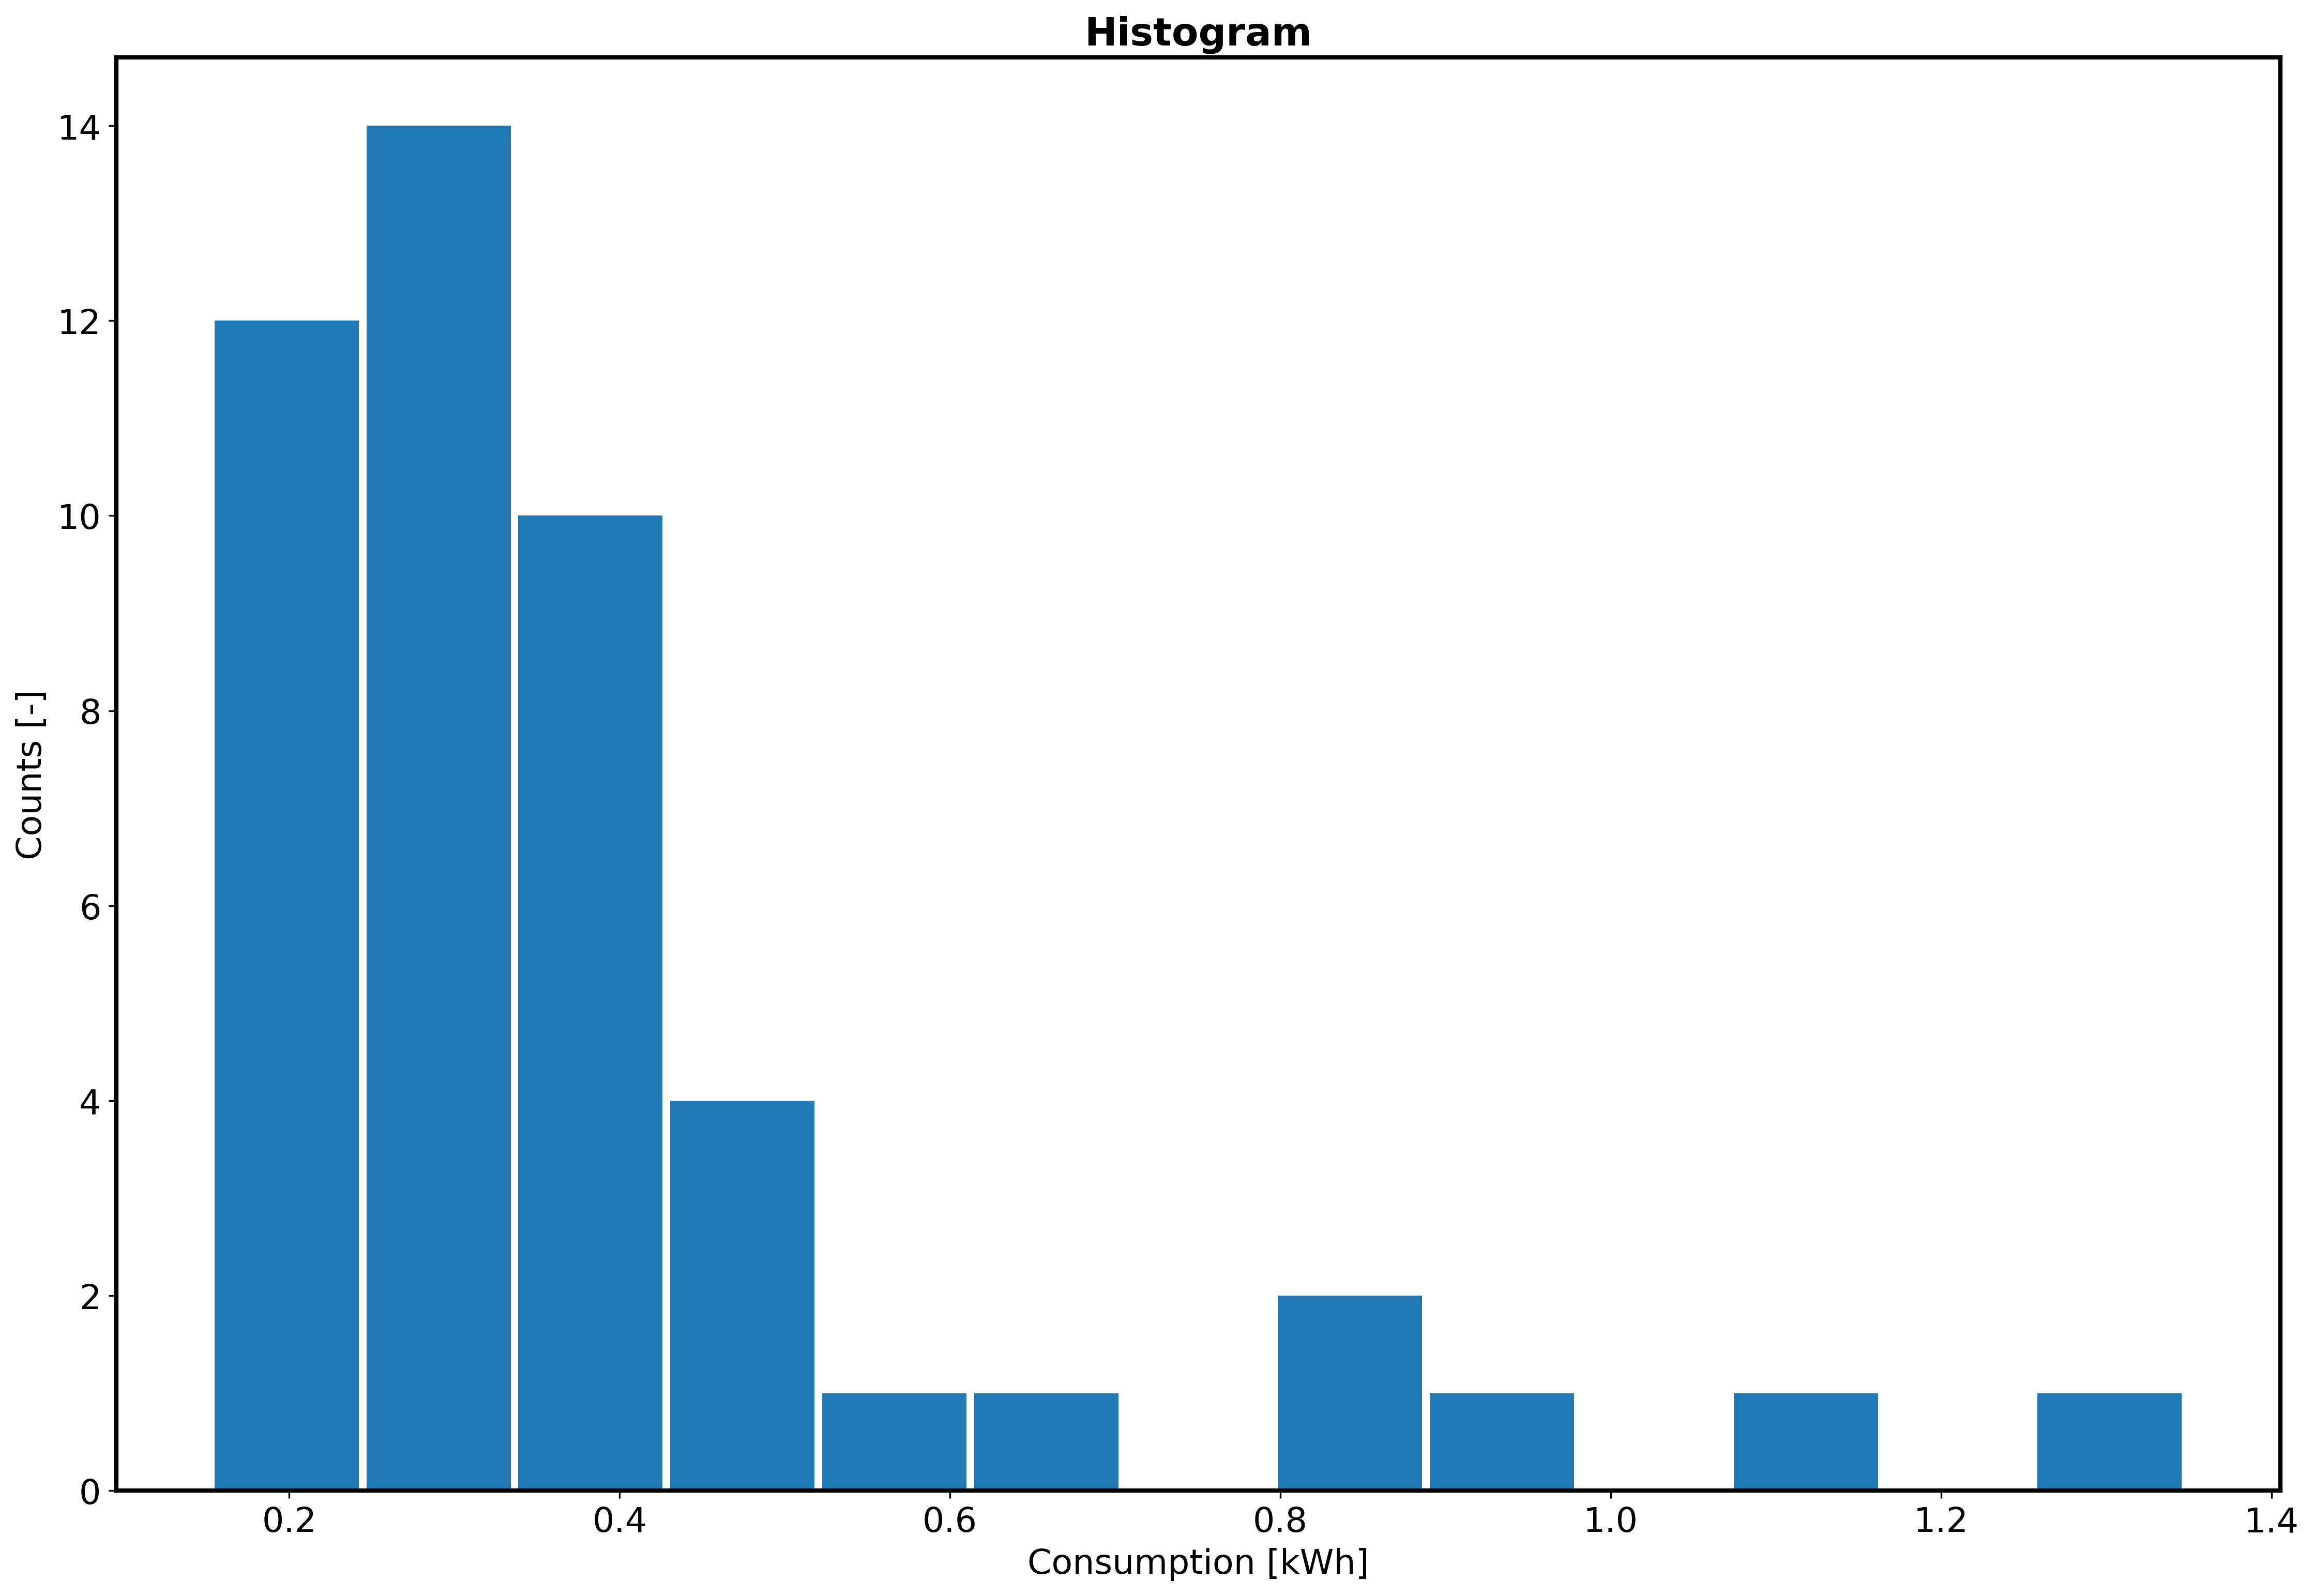
\includegraphics[width=0.8\linewidth]{histogram_mape.png}
	\caption{An example histogram of the consumption in [kWh] versus count [-] used during MAPE forecast.}
	\label{fig:histogram_mape}
\end{figure}

\section{Parameter Search}

\subsection{Model 2}

\begin{table}[h]
	\centering
	\begin{tabular}{@{}l||c|ccc@{}} \toprule
		\multicolumn{5}{c}{Model 2: Stateless (flatten layer)}\\\midrule\midrule
		\textbf{Chosen parameter}	& \textbf{Value} & \textbf{Serie $ 1 $} & \textbf{Serie $ 2 $} & \textbf{Serie $ 3 $}\\\midrule
		Hidden states LSTM & $ 20 $ & $0.446 $&$ 0.0622 $  & \\
		& $ 50 $  & 		  		&		   				& $0.319 $		\\\hline
		layers LSTM & $ 1 $ & 		&		   & 		\\
		& $ 3 $ &  $21.3 $   	&$ 10.60 $  				& $9.98$\\\hline
		Lag value & $ 48 $ & $7.51 $&$ 2.84 $		   & \\
		& $ 96 $ &          		& 		 & 	$1.76$	\\\hline
		Learning rate & $ 10^{-2} $ &       &		 & 		\\
		& $  10^{-3} $ &$23.4 $    &$ 2.51$  			& $13.2$\\
		& $  10^{-4} $ &$43.0 $		&$ 12.8$    	& $17.9$\\\bottomrule
		
	\end{tabular}
	\caption{Each value in this table shows the average error when the corresponding parameter value is used, normalized by the largest error of the possible values of one parameter and finally subtracted by one. Therefore, each value shows a percentage of improvement with respect to the worst value for one parameter for each serie during phase $ 1 $ of the parameter search.}
	\label{tab:relative_performance_parameters_phase_one_model_two}
\end{table}

\begin{table}[h]
	\centering
	\begin{tabular}{@{}l|ccc@{}} \toprule
		\multicolumn{4}{c}{Model 2: Stateless (flatten layer)}\\\midrule\midrule
		\textbf{Parameters}	& \textbf{Serie $ 1 $} & \textbf{Serie $ 2 $} & \textbf{Serie $ 3 $}\\\midrule
		Hidden states LSTM & $20 $&$ 50 $  & $50 $\\
		layers LSTM & $3 $&$ 3 $  & $3$\\
		Lag value & $96 $&$ 48$  & $96$\\
		Learning rate & $0.001 $&$ 0.0001$  & $0.001$\\\hline
		MAE error 1   & $ 0.137 $ & $ 0.0426 $ & $ 0.0973 $\\
		MAE error 2   & $ 0.139 $ & $ 0.0430 $ & $ 0.107 $\\
		MAE error 3   & $ 0.136 $ & $ 0.0424 $ & $ 0.100 $\\\bottomrule
	\end{tabular}
	\caption{The values of the parameters with the lowest average MAE on the validation set over three runs.}
	\label{tab:best_performing_para_phase1_model2}
\end{table}


\begin{figure}[h]
	\centering
	\begin{subfigure}{0.49\linewidth}
		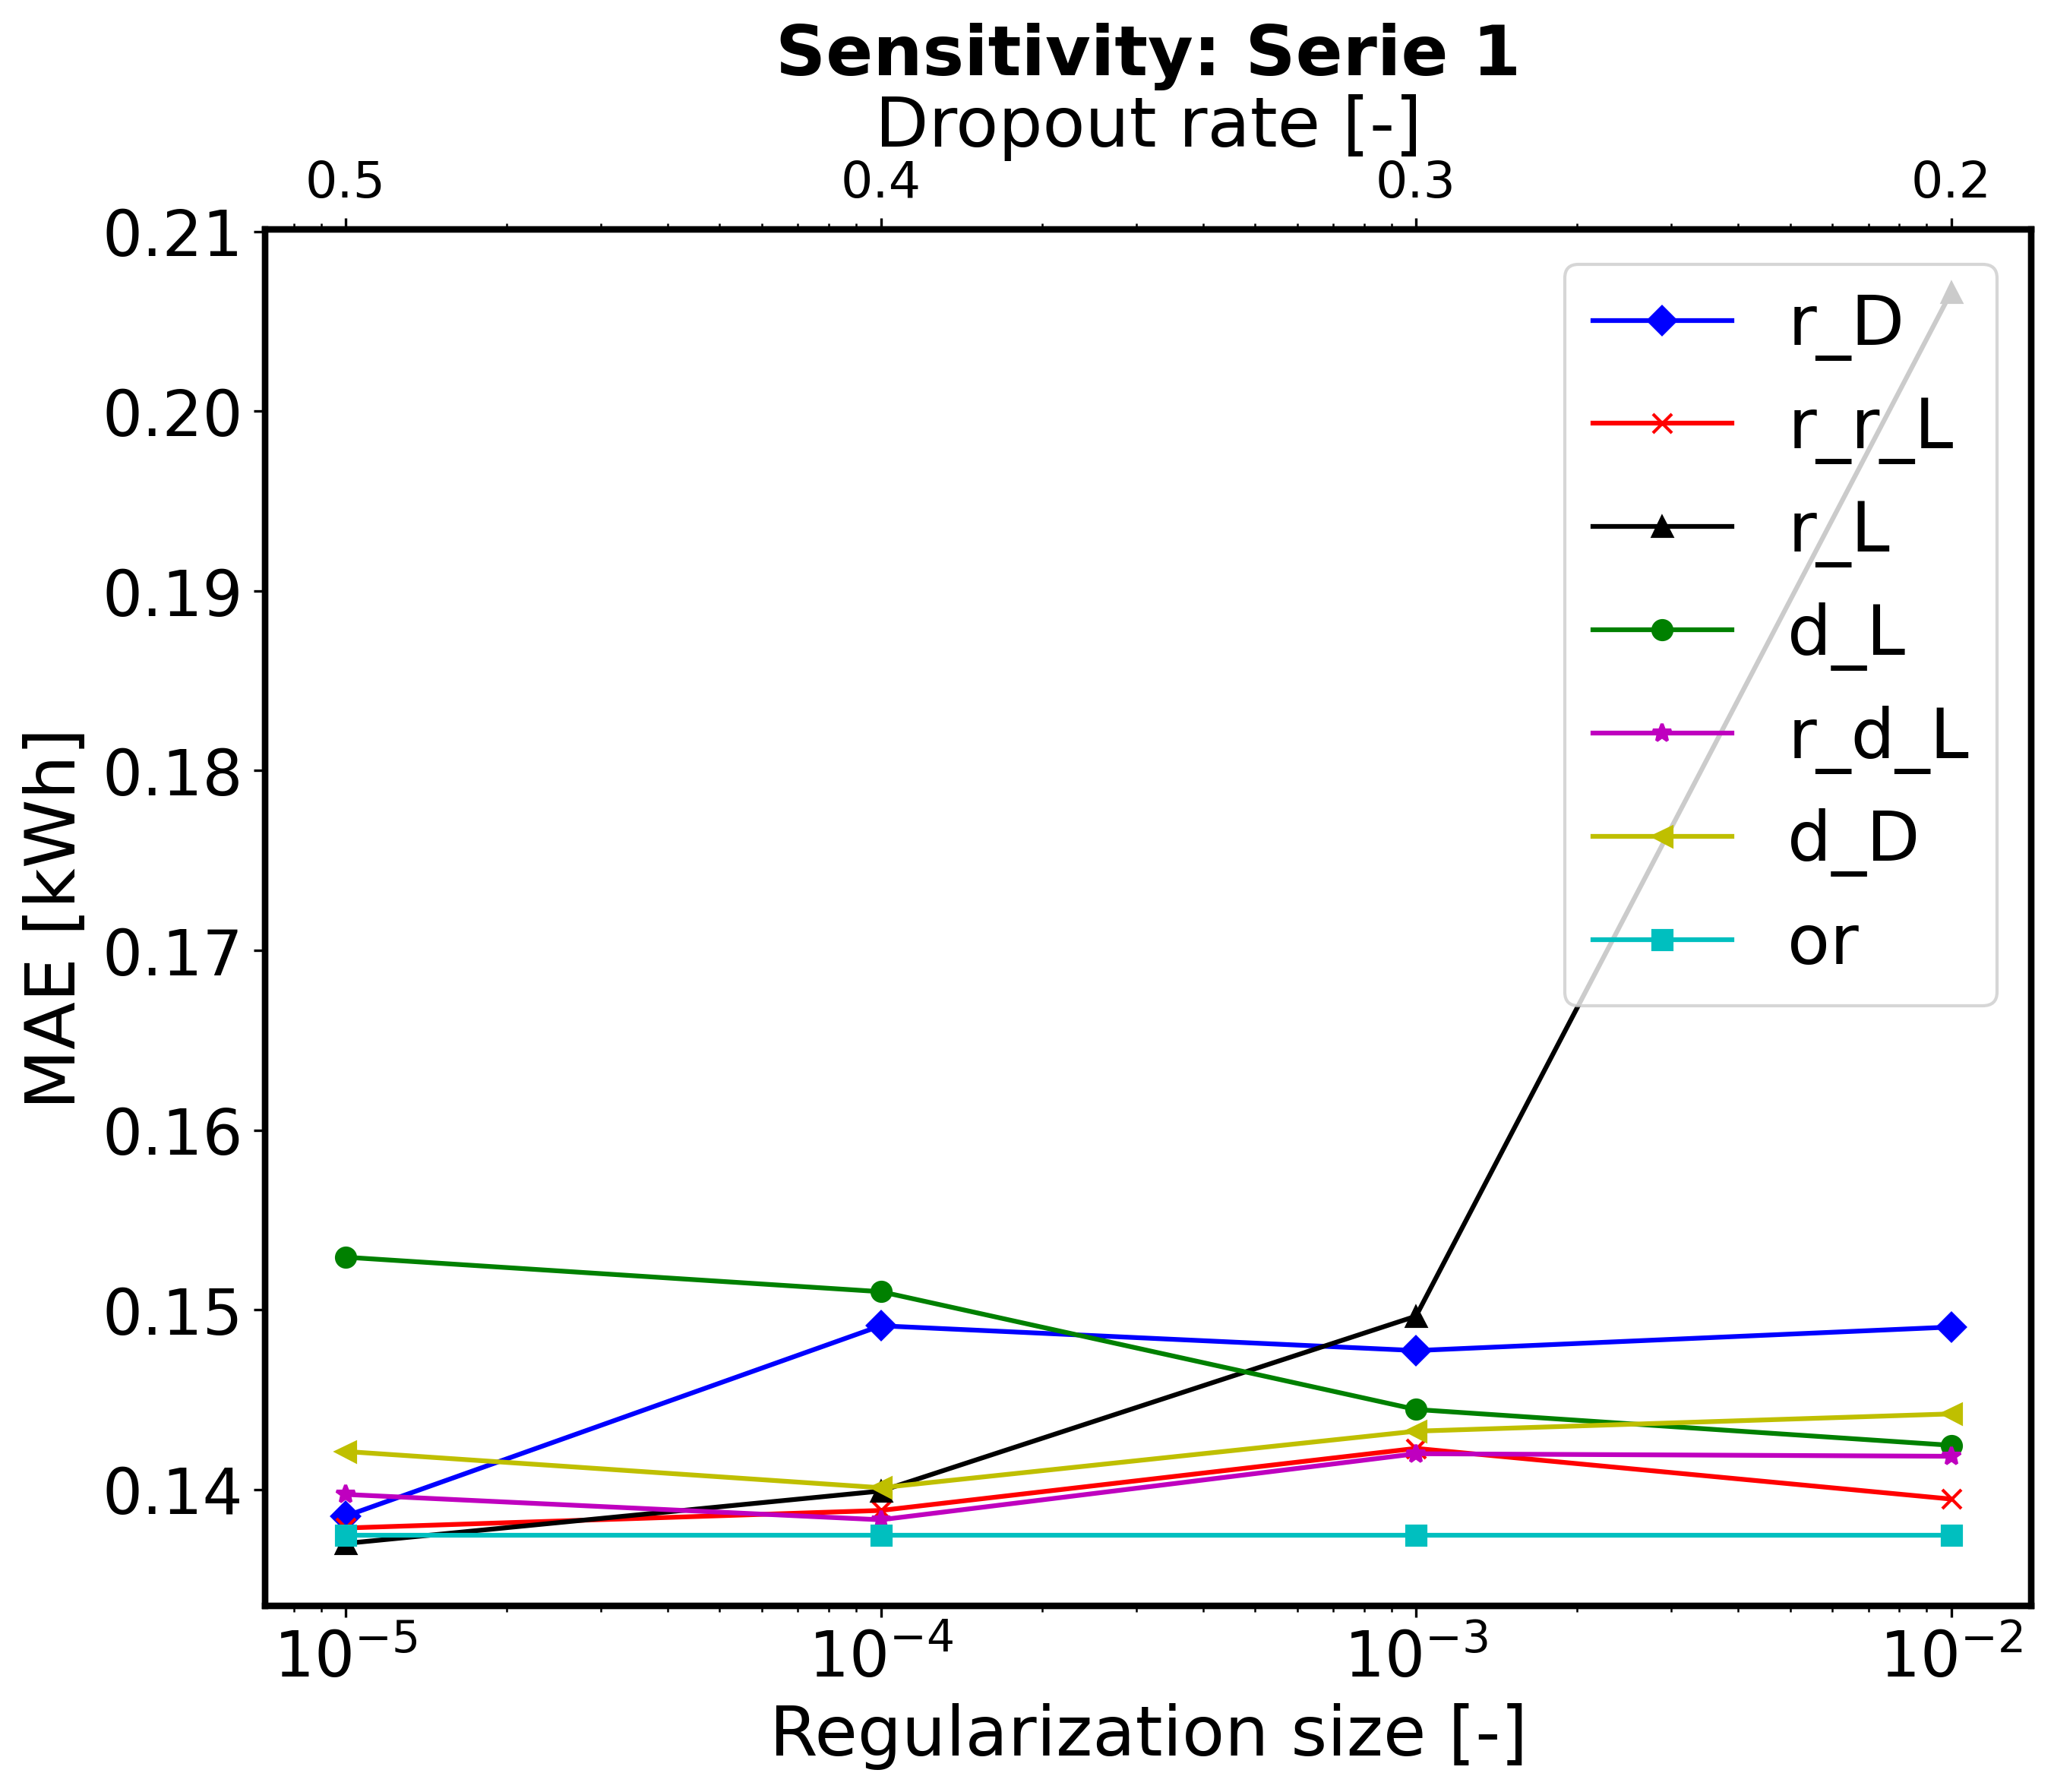
\includegraphics[width=1\linewidth]{serie1_model2.png}
		\caption{Model 2}
	\end{subfigure}	
	\begin{subfigure}{0.49\linewidth}
		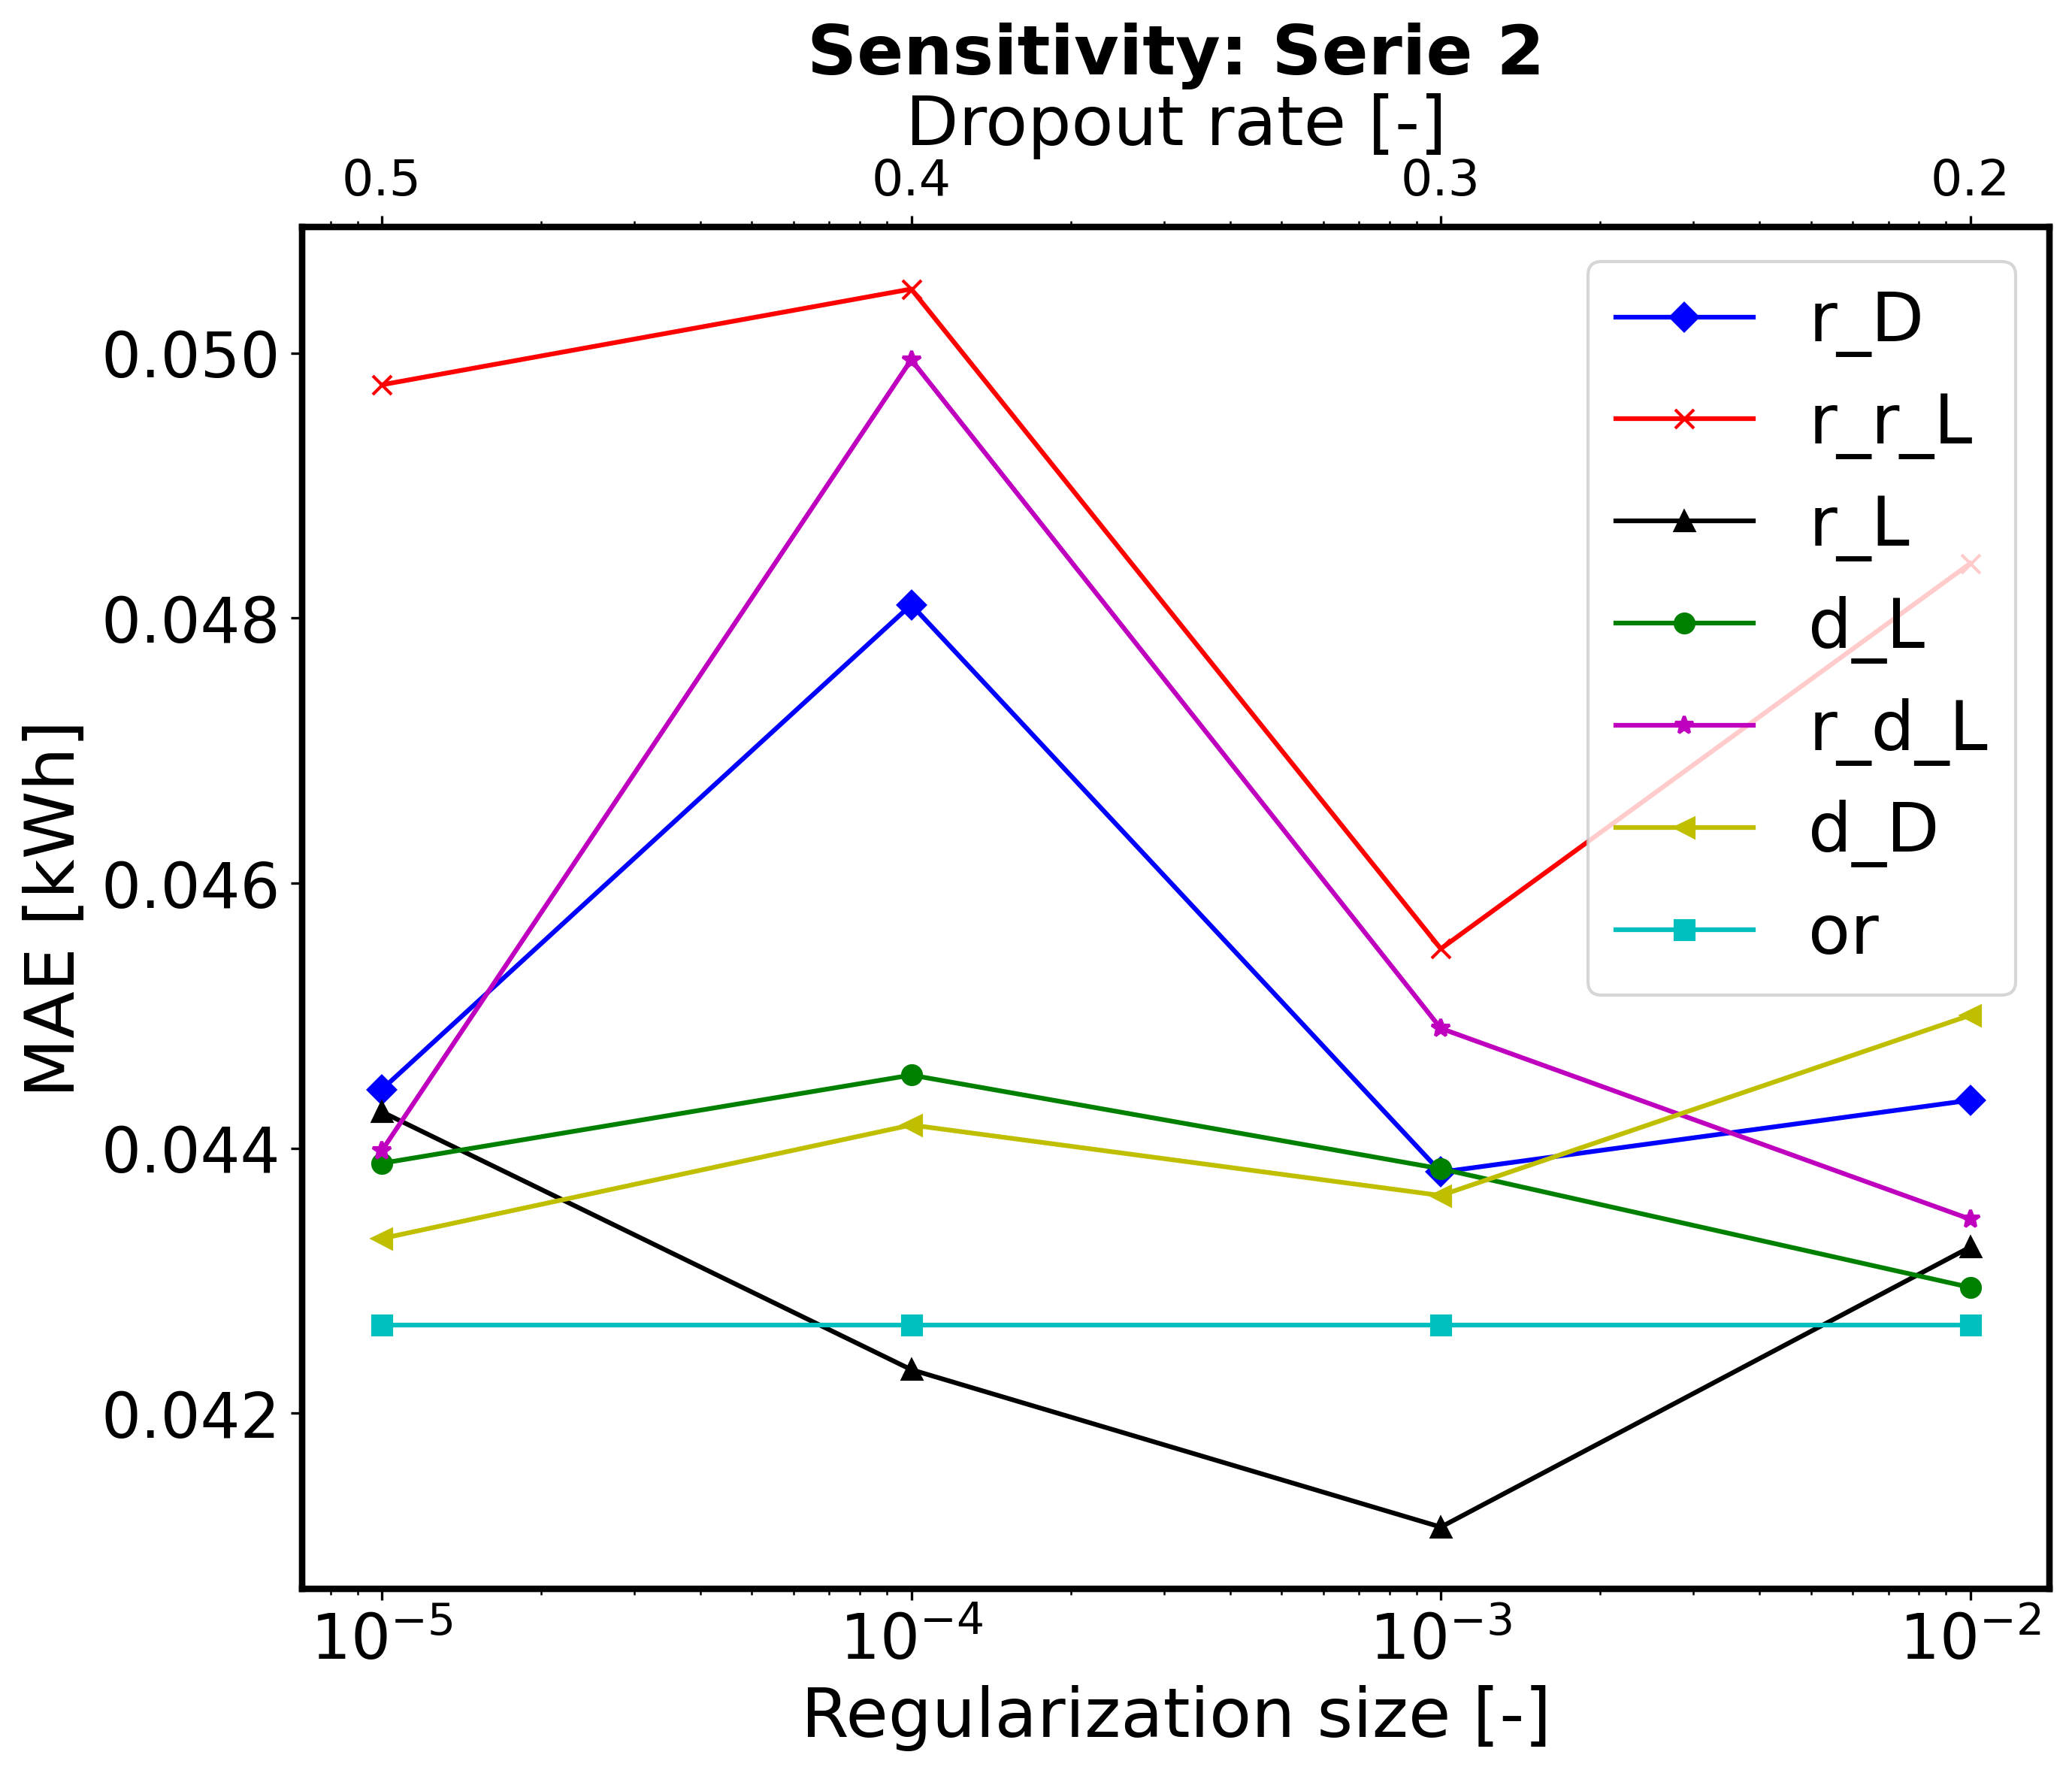
\includegraphics[width=1\linewidth]{serie2_model2.png}
		\caption{Model 2}
	\end{subfigure}
	\begin{subfigure}{0.5\linewidth}
		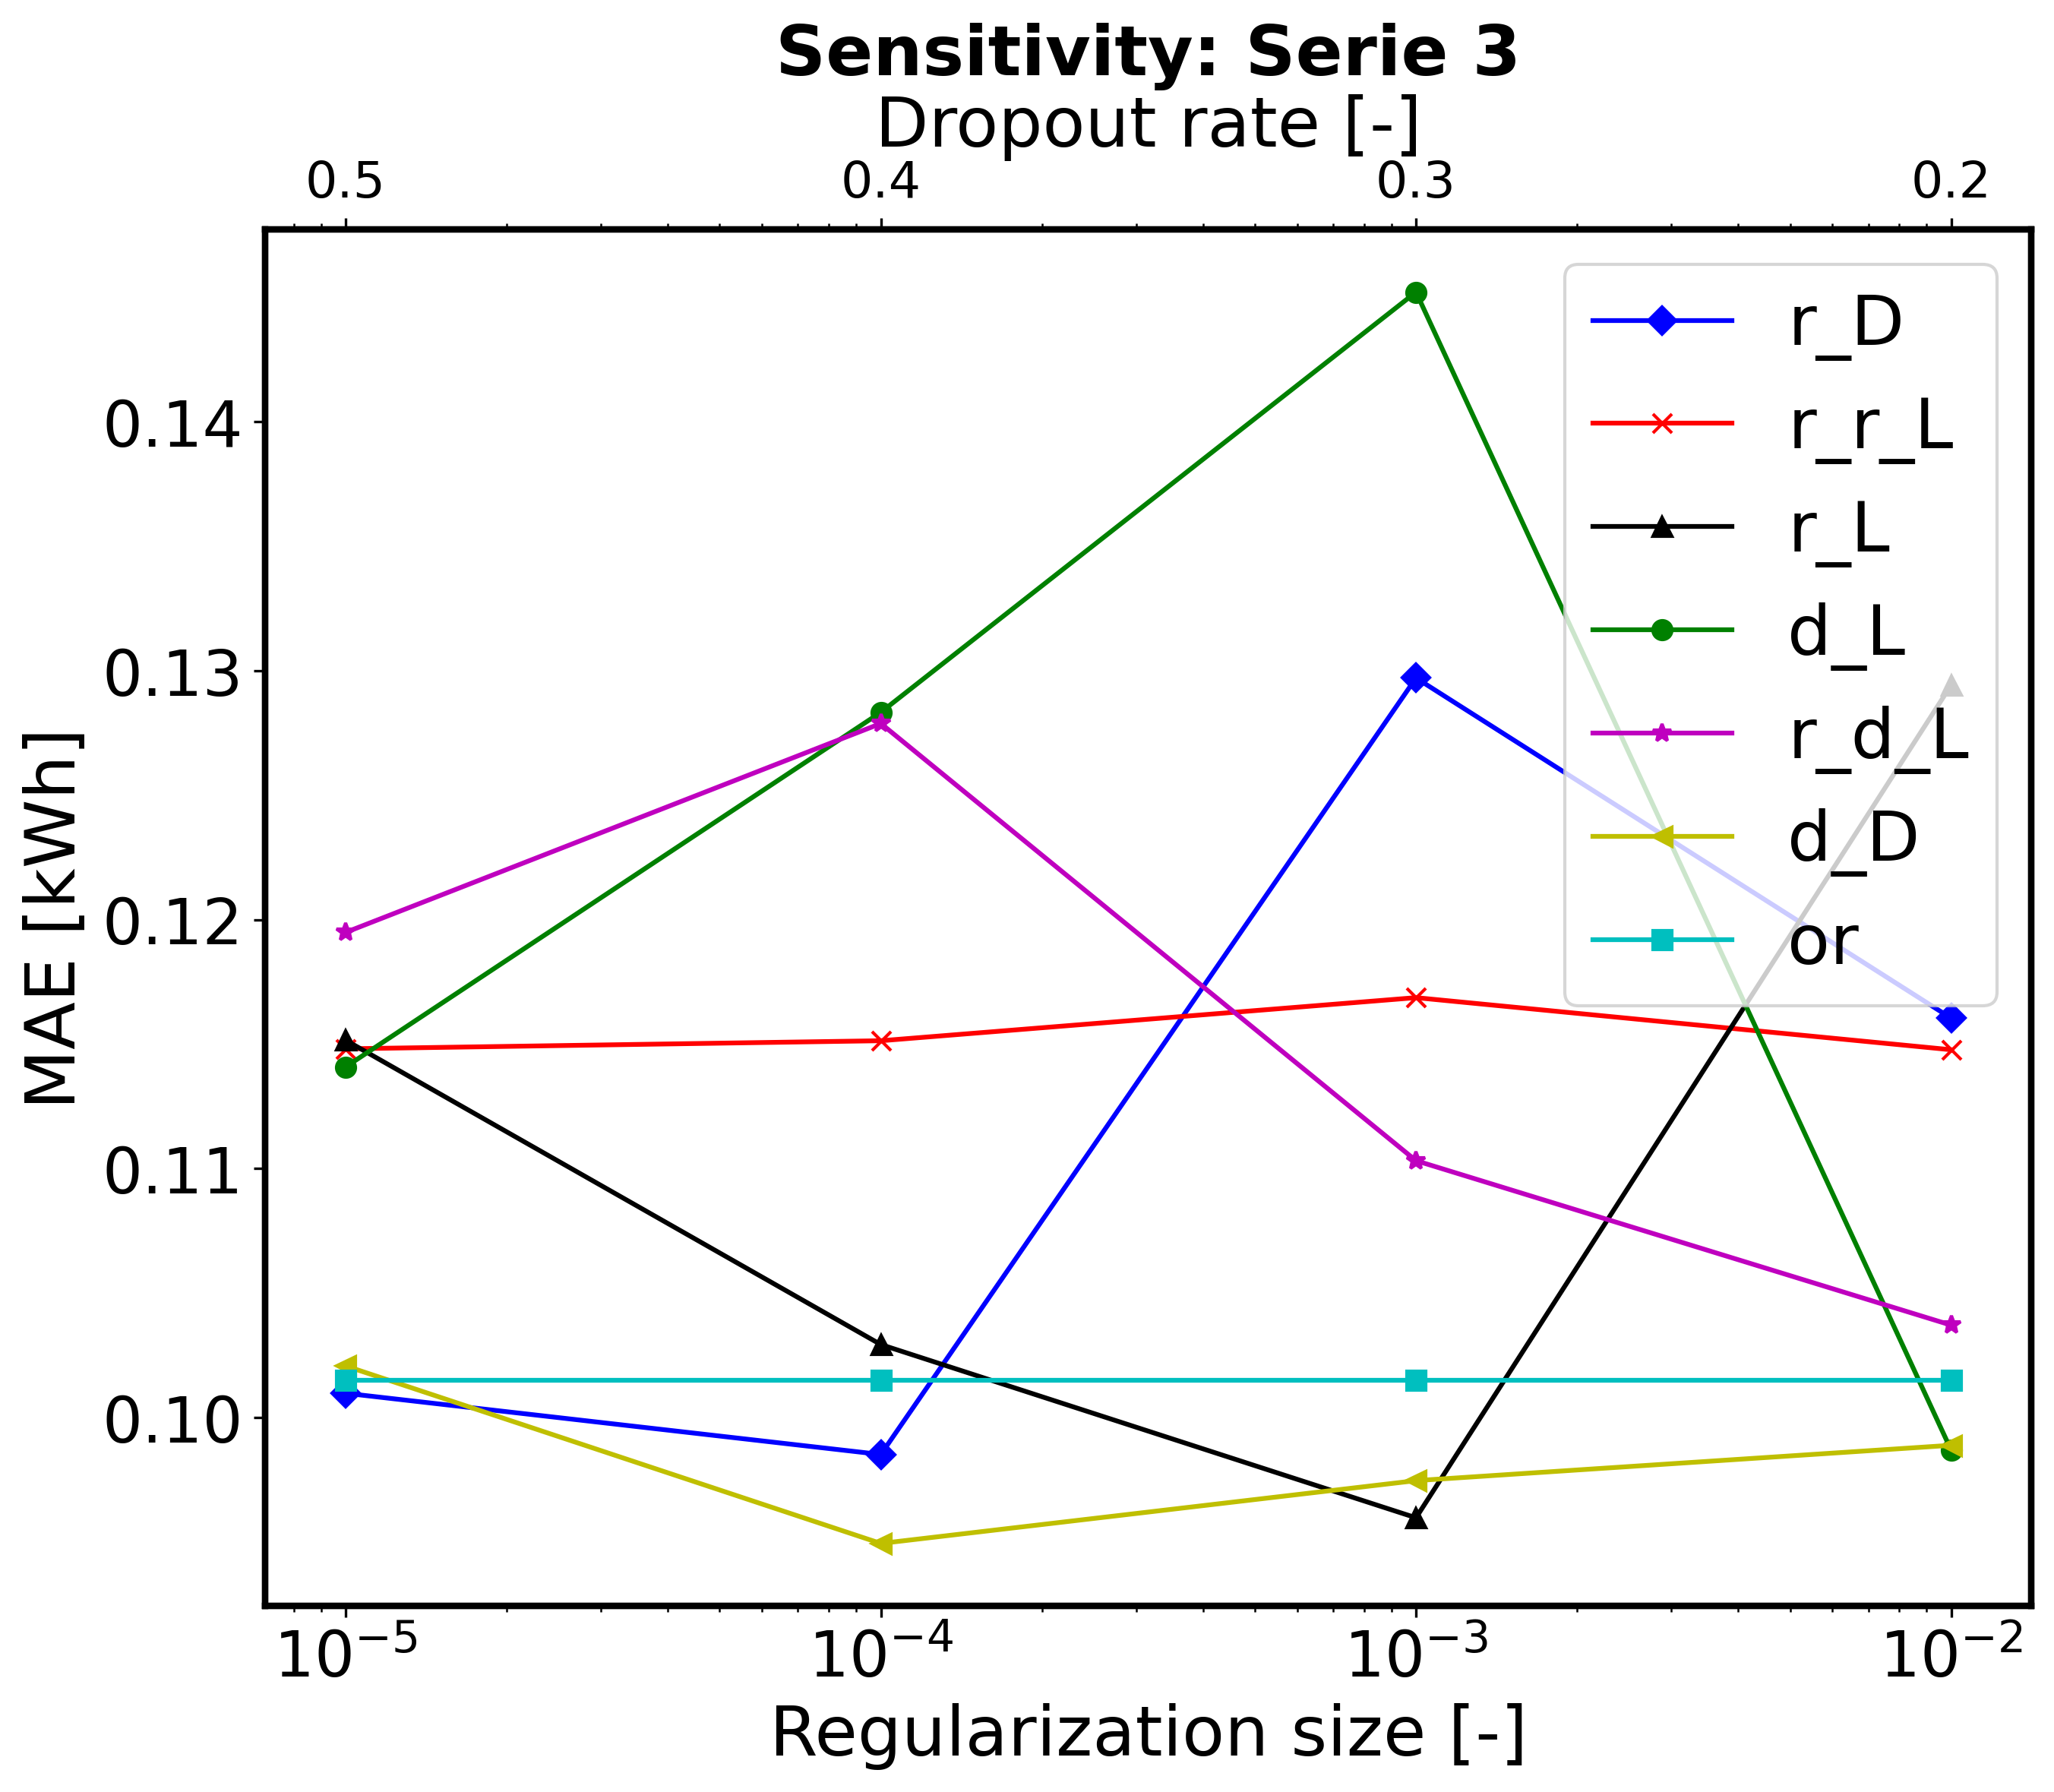
\includegraphics[width=1\linewidth]{serie3_model2.png}
		\caption{Model 2}
	\end{subfigure}
	\caption{Results of the sensitivity analysis on the size of the regularization parameter and the dropout rate according to MAE.(Legend: \textit{r\_D}: regularization size of weights of DENSE layer,  \textit{r\_r\_L}: regularization size of recurrent weight of LSTM, \textit{r\_L}: regularization size of input weights of LSTM, \textit{d\_L}: dropout rate of inputs LSTM, \textit{r\_d\_L}: dropout rate of hidden states LSTM, \textit{d\_D}: dropout rate of DENSE layer, \textit{or}: best performing serie from phase one)}
	\label{fig:sensitivity_model2}
\end{figure}

\begin{figure}[h]
	\centering
	\begin{subfigure}{0.49\linewidth}
		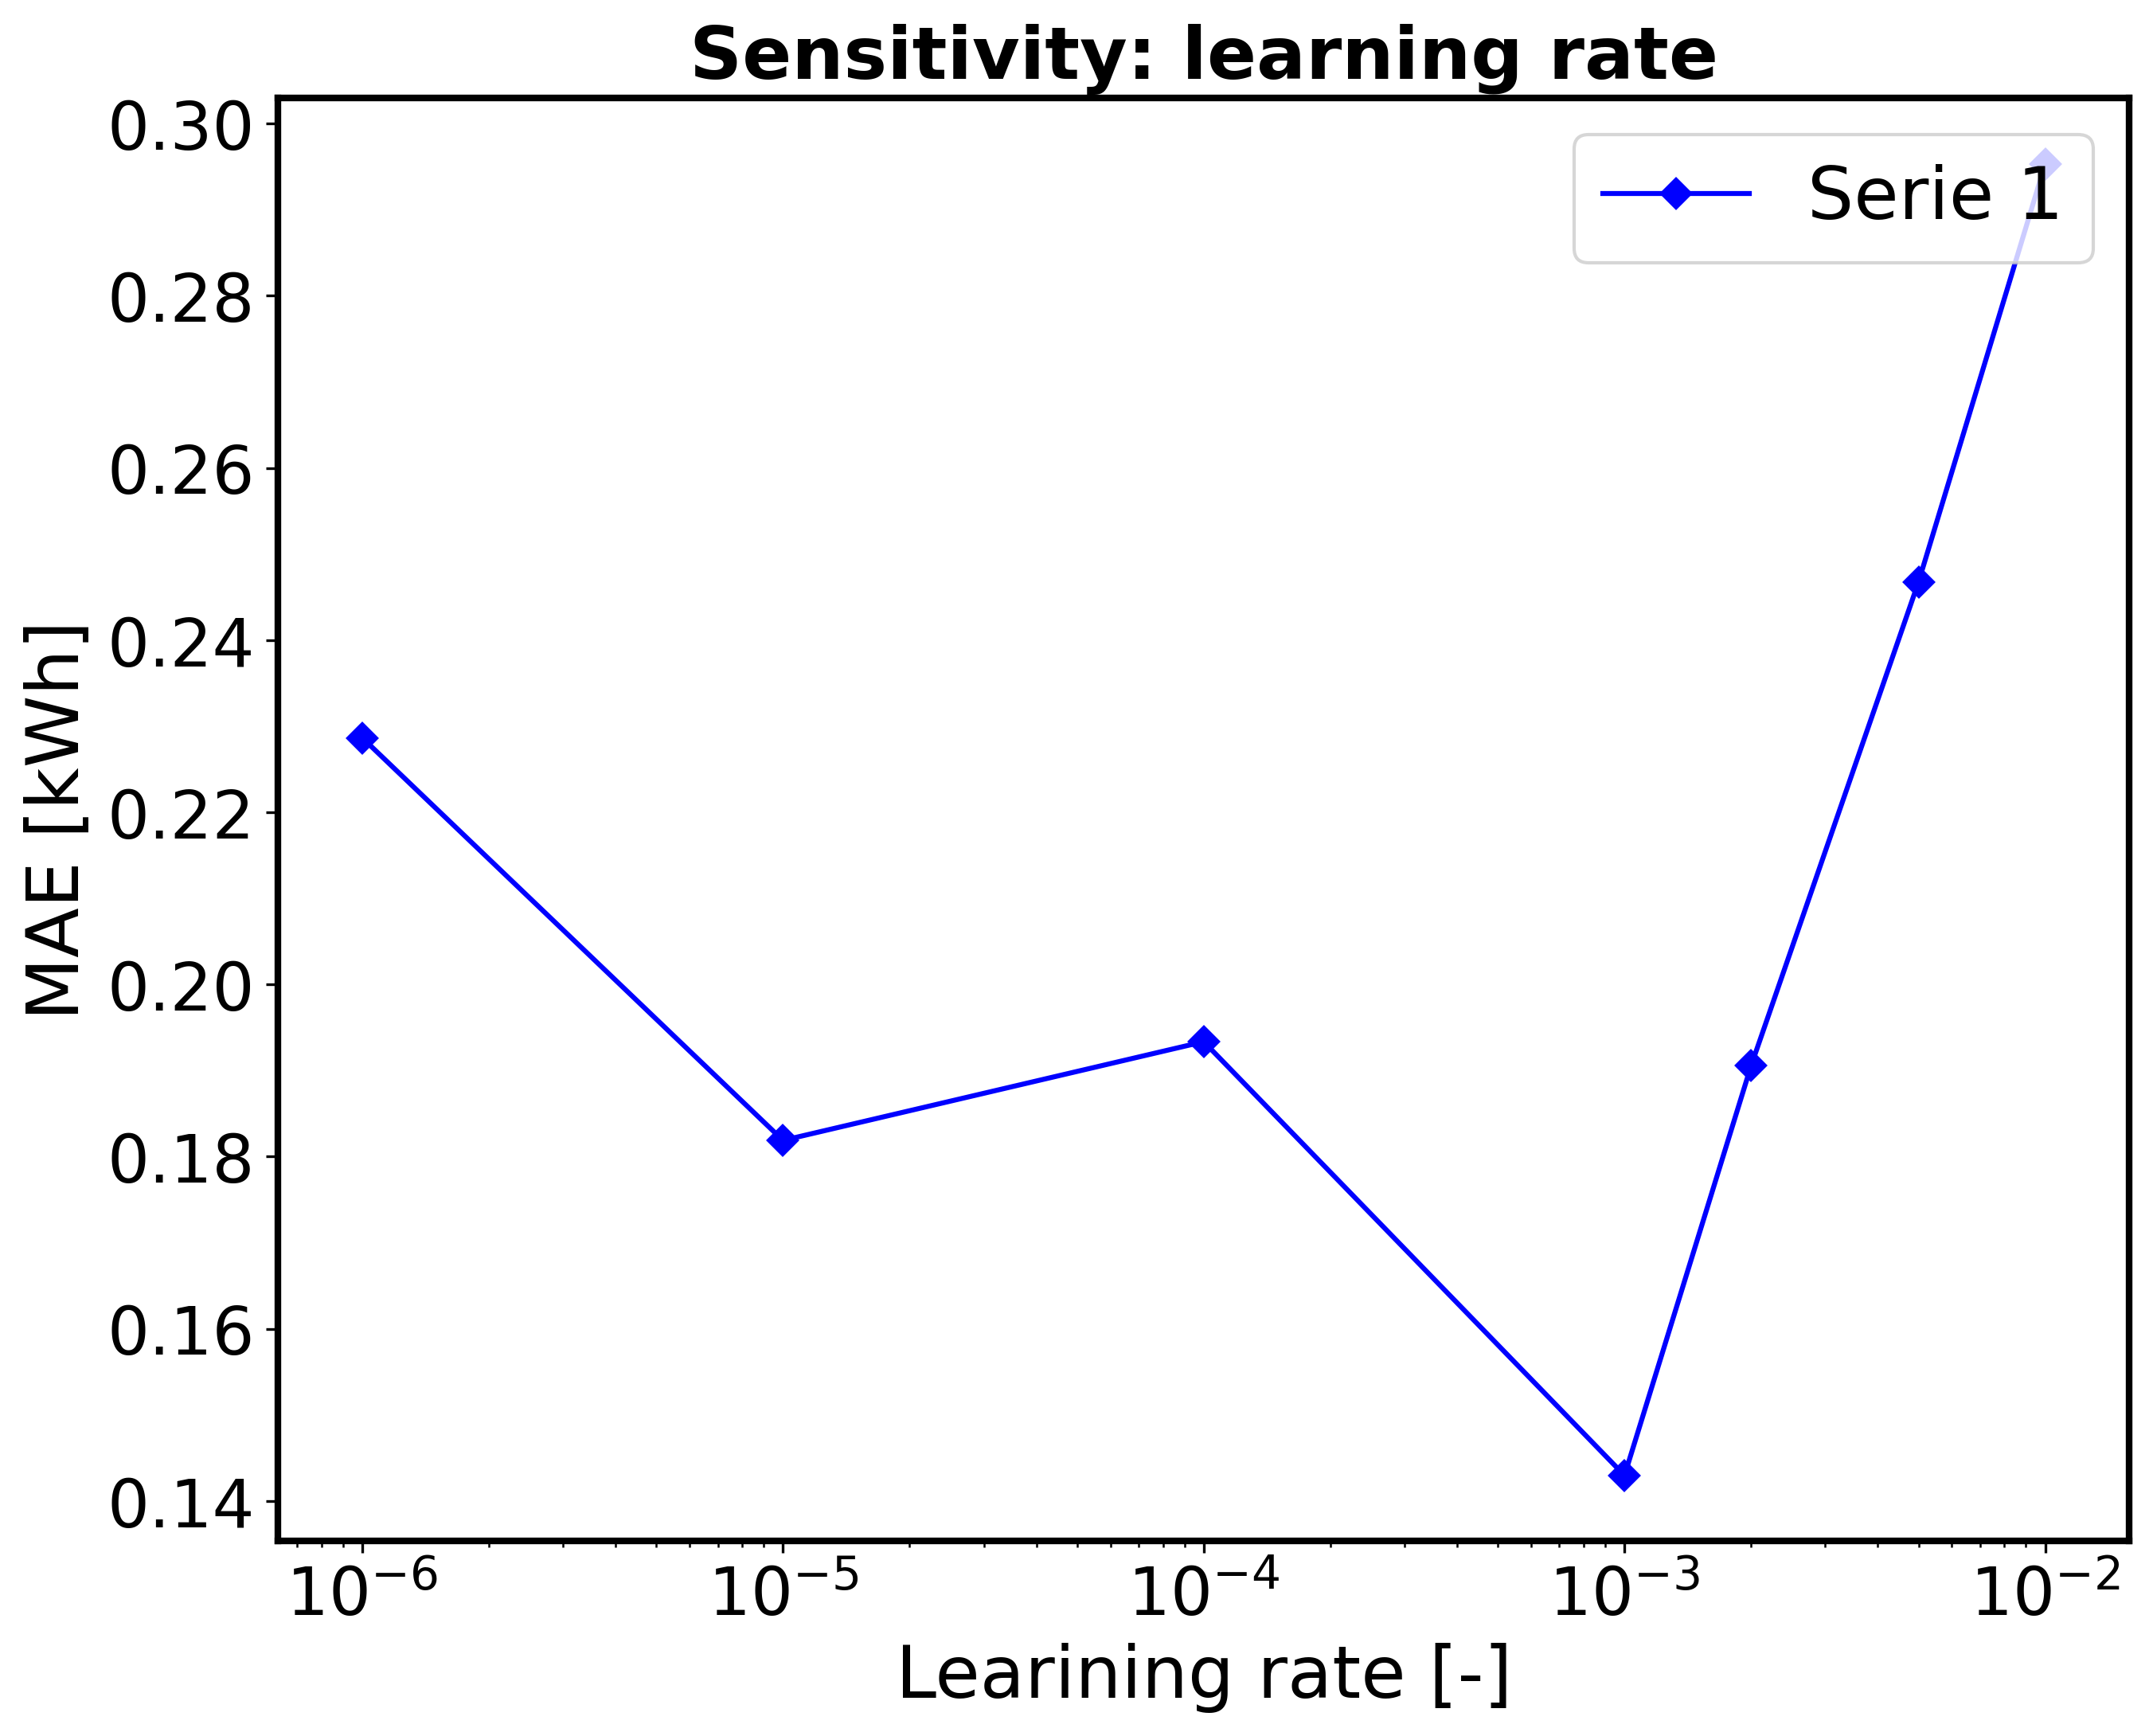
\includegraphics[width=1\linewidth]{learning_rate_serie1_model2.png}
		\caption{Model 2}
	\end{subfigure}	
	\begin{subfigure}{0.49\linewidth}
		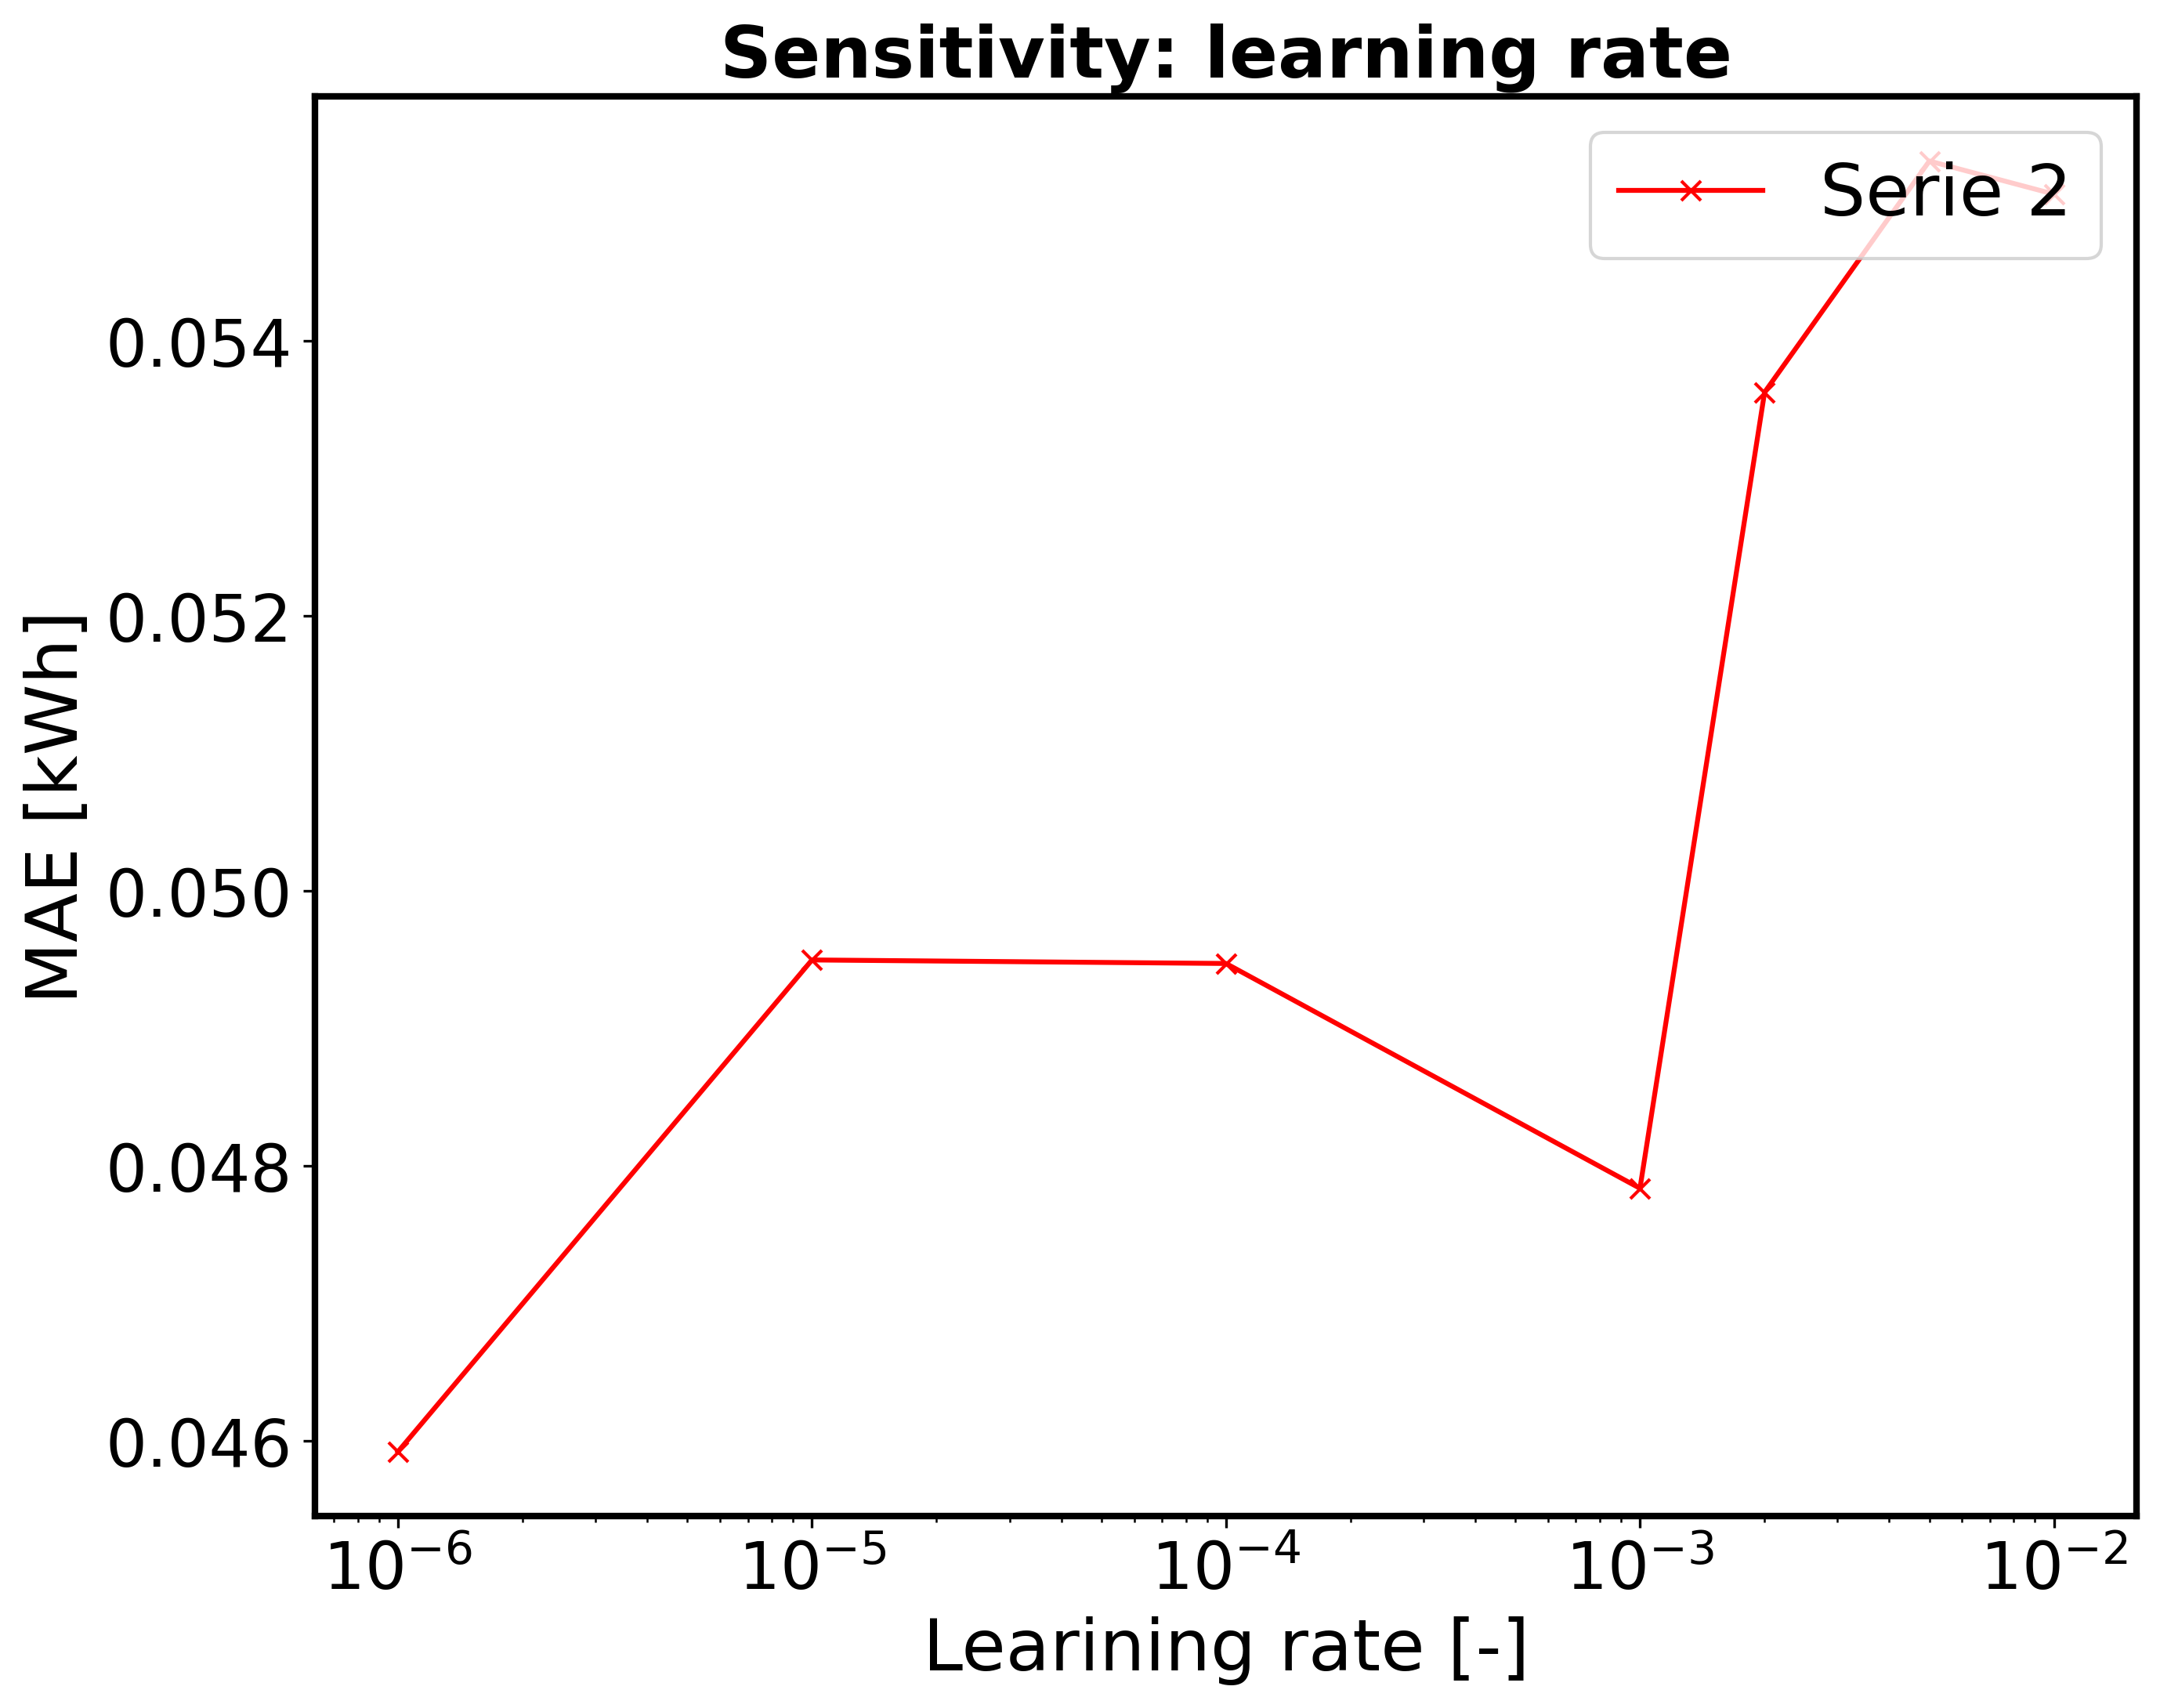
\includegraphics[width=1\linewidth]{learning_rate_serie2_model2.png}
		\caption{Model 2}
	\end{subfigure}
	\begin{subfigure}{0.5\linewidth}
		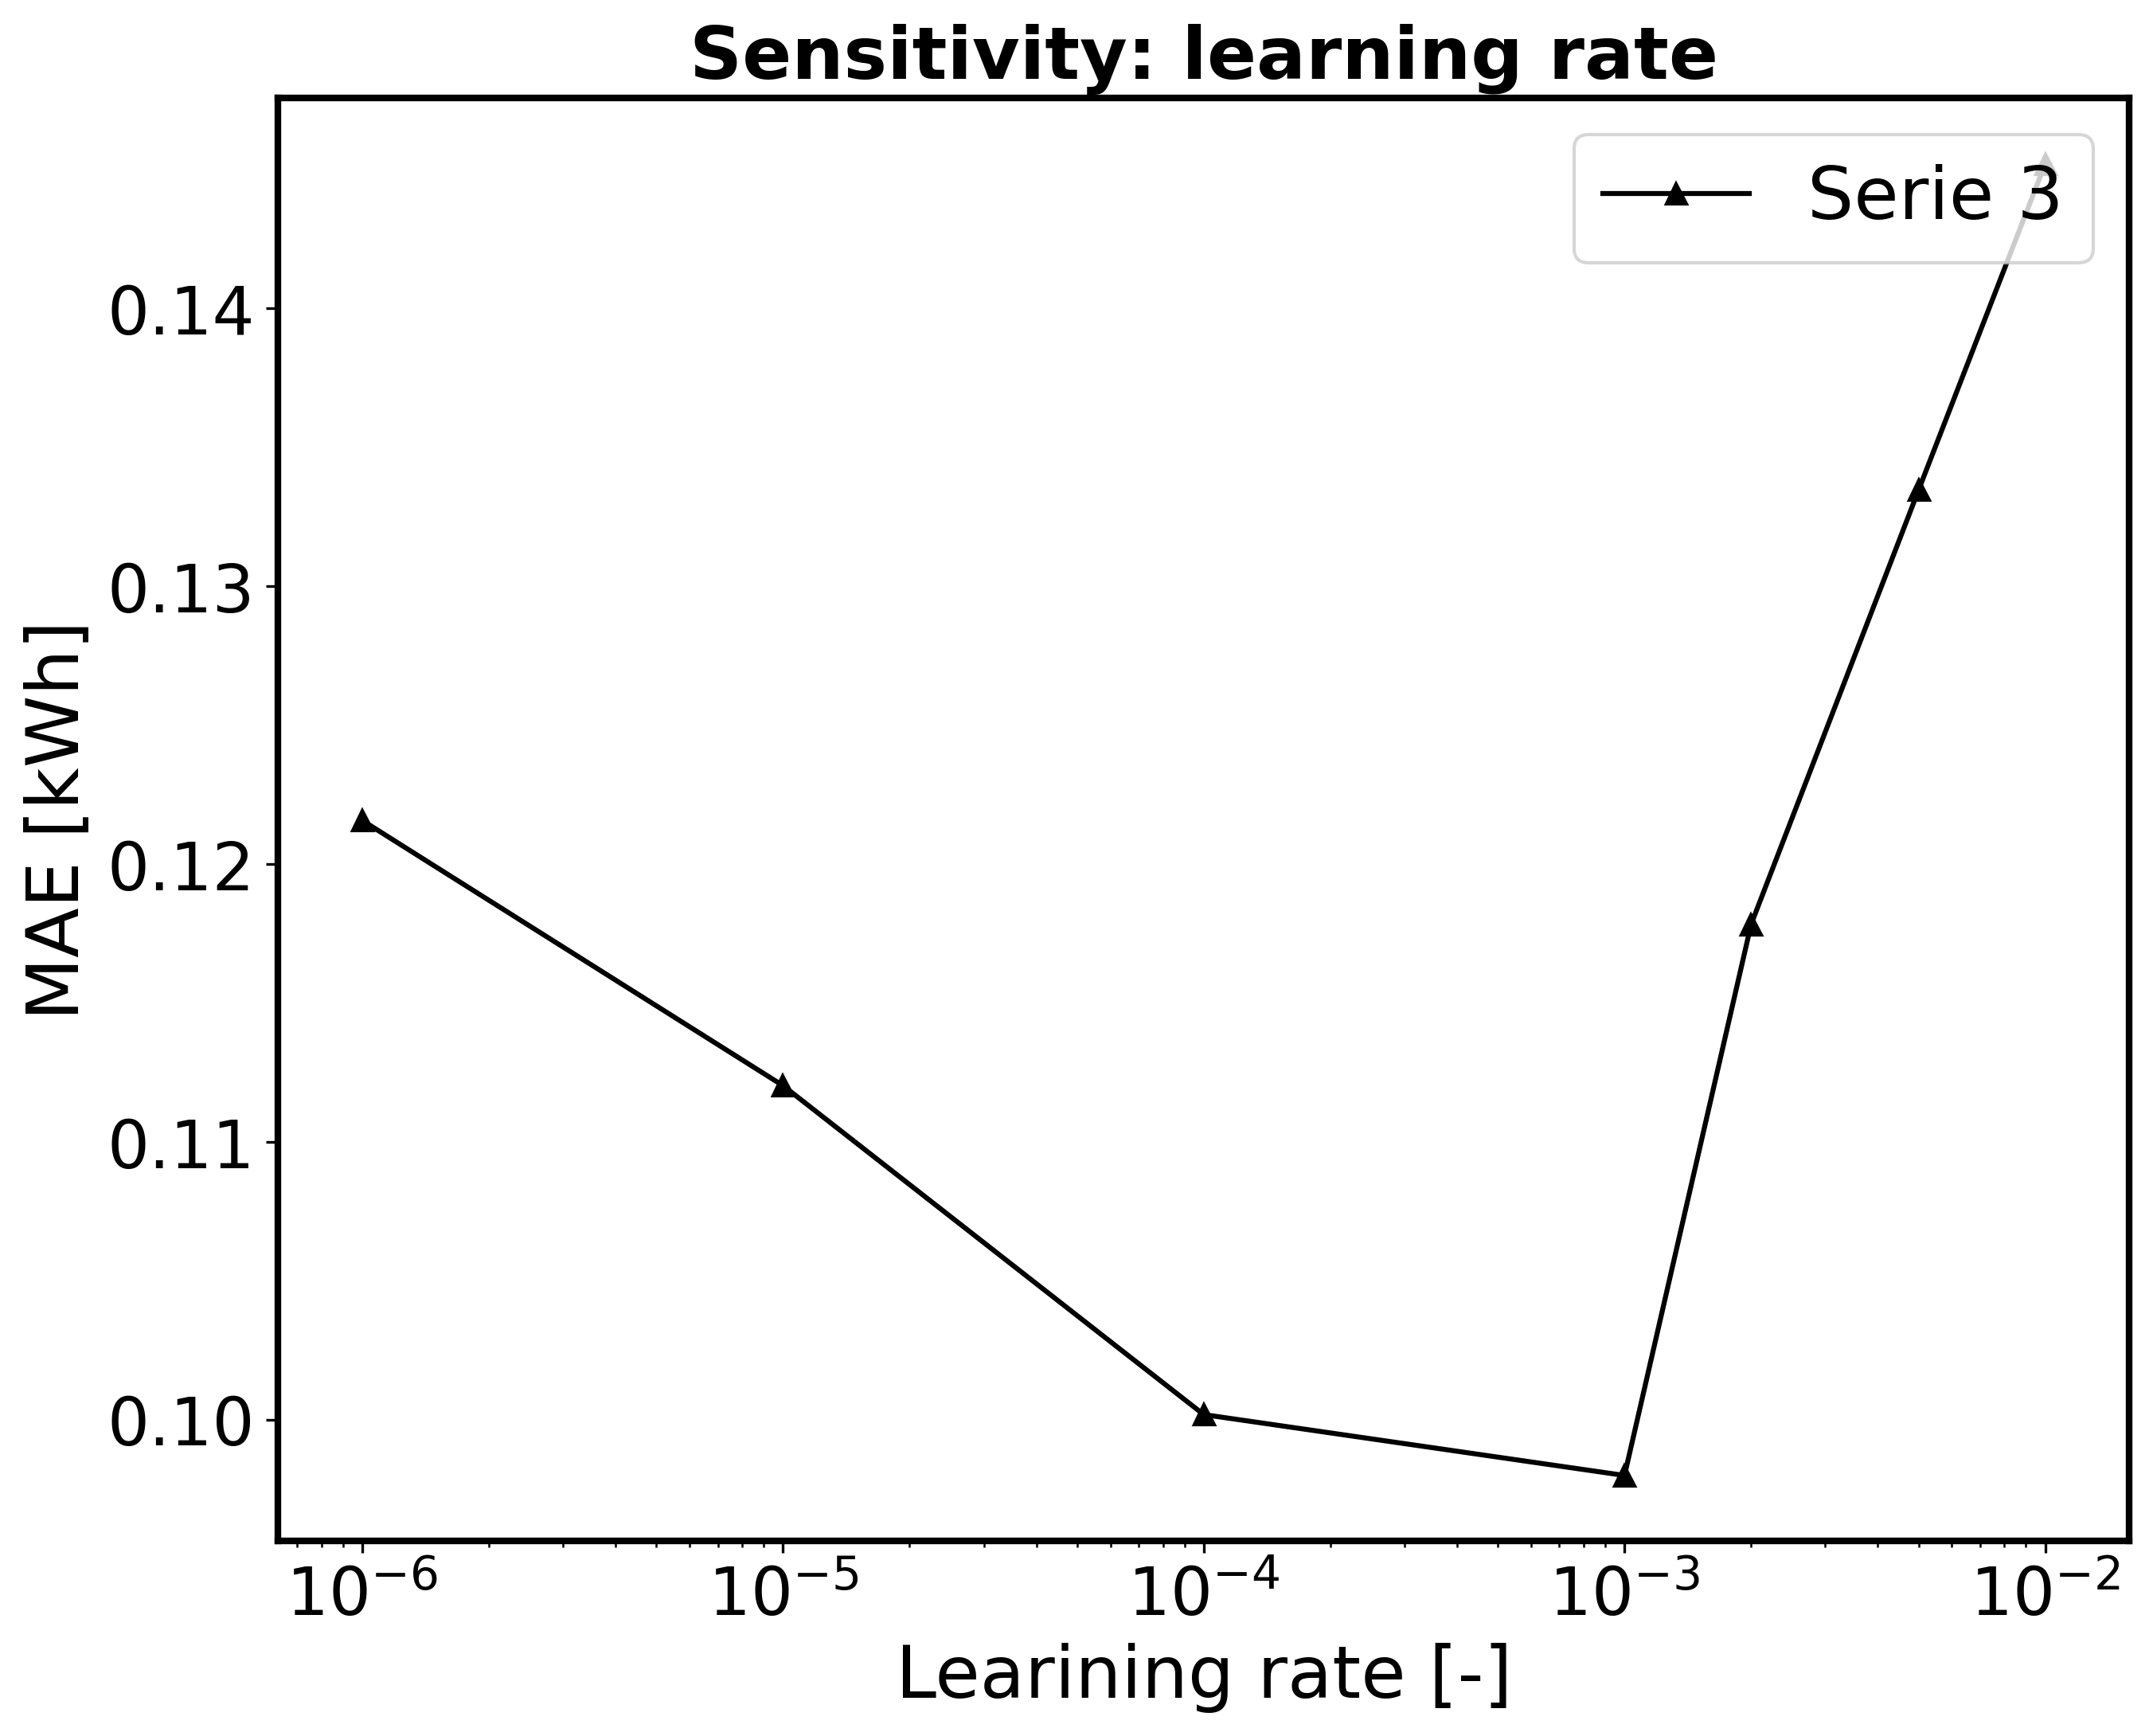
\includegraphics[width=1\linewidth]{learning_rate_serie3_model2.png}
		\caption{Model 2}
	\end{subfigure}
	\caption{The evaluation of the error on the validation set in function of the learning rate size.}
	\label{fig:learning_rate_model2}
\end{figure}

\clearpage
\subsection{Model 3}

\begin{table}[ht]
	\centering
	\begin{tabular}{@{}l||c|ccc@{}} \toprule
		\multicolumn{5}{c}{Model 3: Stateful (1 time step)}\\\midrule\midrule
		\textbf{Chosen parameter}	& \textbf{Value} & \textbf{Serie $ 1 $} & \textbf{Serie $ 2 $} & \textbf{Serie $ 3 $}\\\midrule
		Hidden states LSTM & $ 20 $ & $6.66 $		&  & $0.55 $\\
		& $ 50 $ & 		  		&	$ 0.51 $	   & 		\\\hline
		layers LSTM & $ 1 $ & $30.00 $		&	$ 1.52 $	   & 	$7.42$	\\
		& $ 3 $ & 	      		& 			 & \\\hline
		Learning rate & $ 10^{-2} $ &       &		   & 		\\
		& $  10^{-3} $ &$17.72 $&$0.0$  & $0.0$\\
		& $  10^{-4} $ &$27.28 $&$ 2.28$    & $11.13$\\\bottomrule
		
	\end{tabular}
	\caption{Each value in this table shows the average error when the corresponding parameter value is used, normalized by the largest error of the possible values of one parameter and finally subtracted by one. Therefore, each value shows a percentage of improvement with respect to the worst value for one parameter for each serie during phase $ 1 $ of the parameter search.}
	\label{tab:relative_performance_parameters_phase_one_model_three}
\end{table}

\begin{table}[ht]
	\centering
	\begin{tabular}{@{}l|ccc@{}} \toprule
		\multicolumn{4}{c}{Model 3: Stateful (1 time step)}\\\midrule\midrule
		\textbf{Parameters}	& \textbf{Serie $ 1 $} & \textbf{Serie $ 2 $} & \textbf{Serie $ 3 $}\\\midrule
		Hidden states LSTM  & $50 $&$ 50 $  & $20 $\\
		layers LSTM & $1 $&$ 1 $  & $1$\\
		Learning rate & $0.0001 $&$ 0.0001$  & $0.0001$\\\hline
		MAE error 1   & $ 0.132 $ & $ 0.0522 $ & $ 0.109 $\\
		MAE error 2   & $ 0.130 $ & $ 0.0613 $ & $ 0.111 $\\
		MAE error 3   & $ 0.138 $ & $ 0.0570 $ & $ 0.112 $\\\bottomrule
	\end{tabular}
	\caption{The values of the parameters with the lowest average MAE on the validation set over three runs.}
	\label{tab:best_performing_para_phase1_model3}
\end{table}

\begin{figure}[ht]
	\centering
	\begin{subfigure}{0.49\linewidth}
		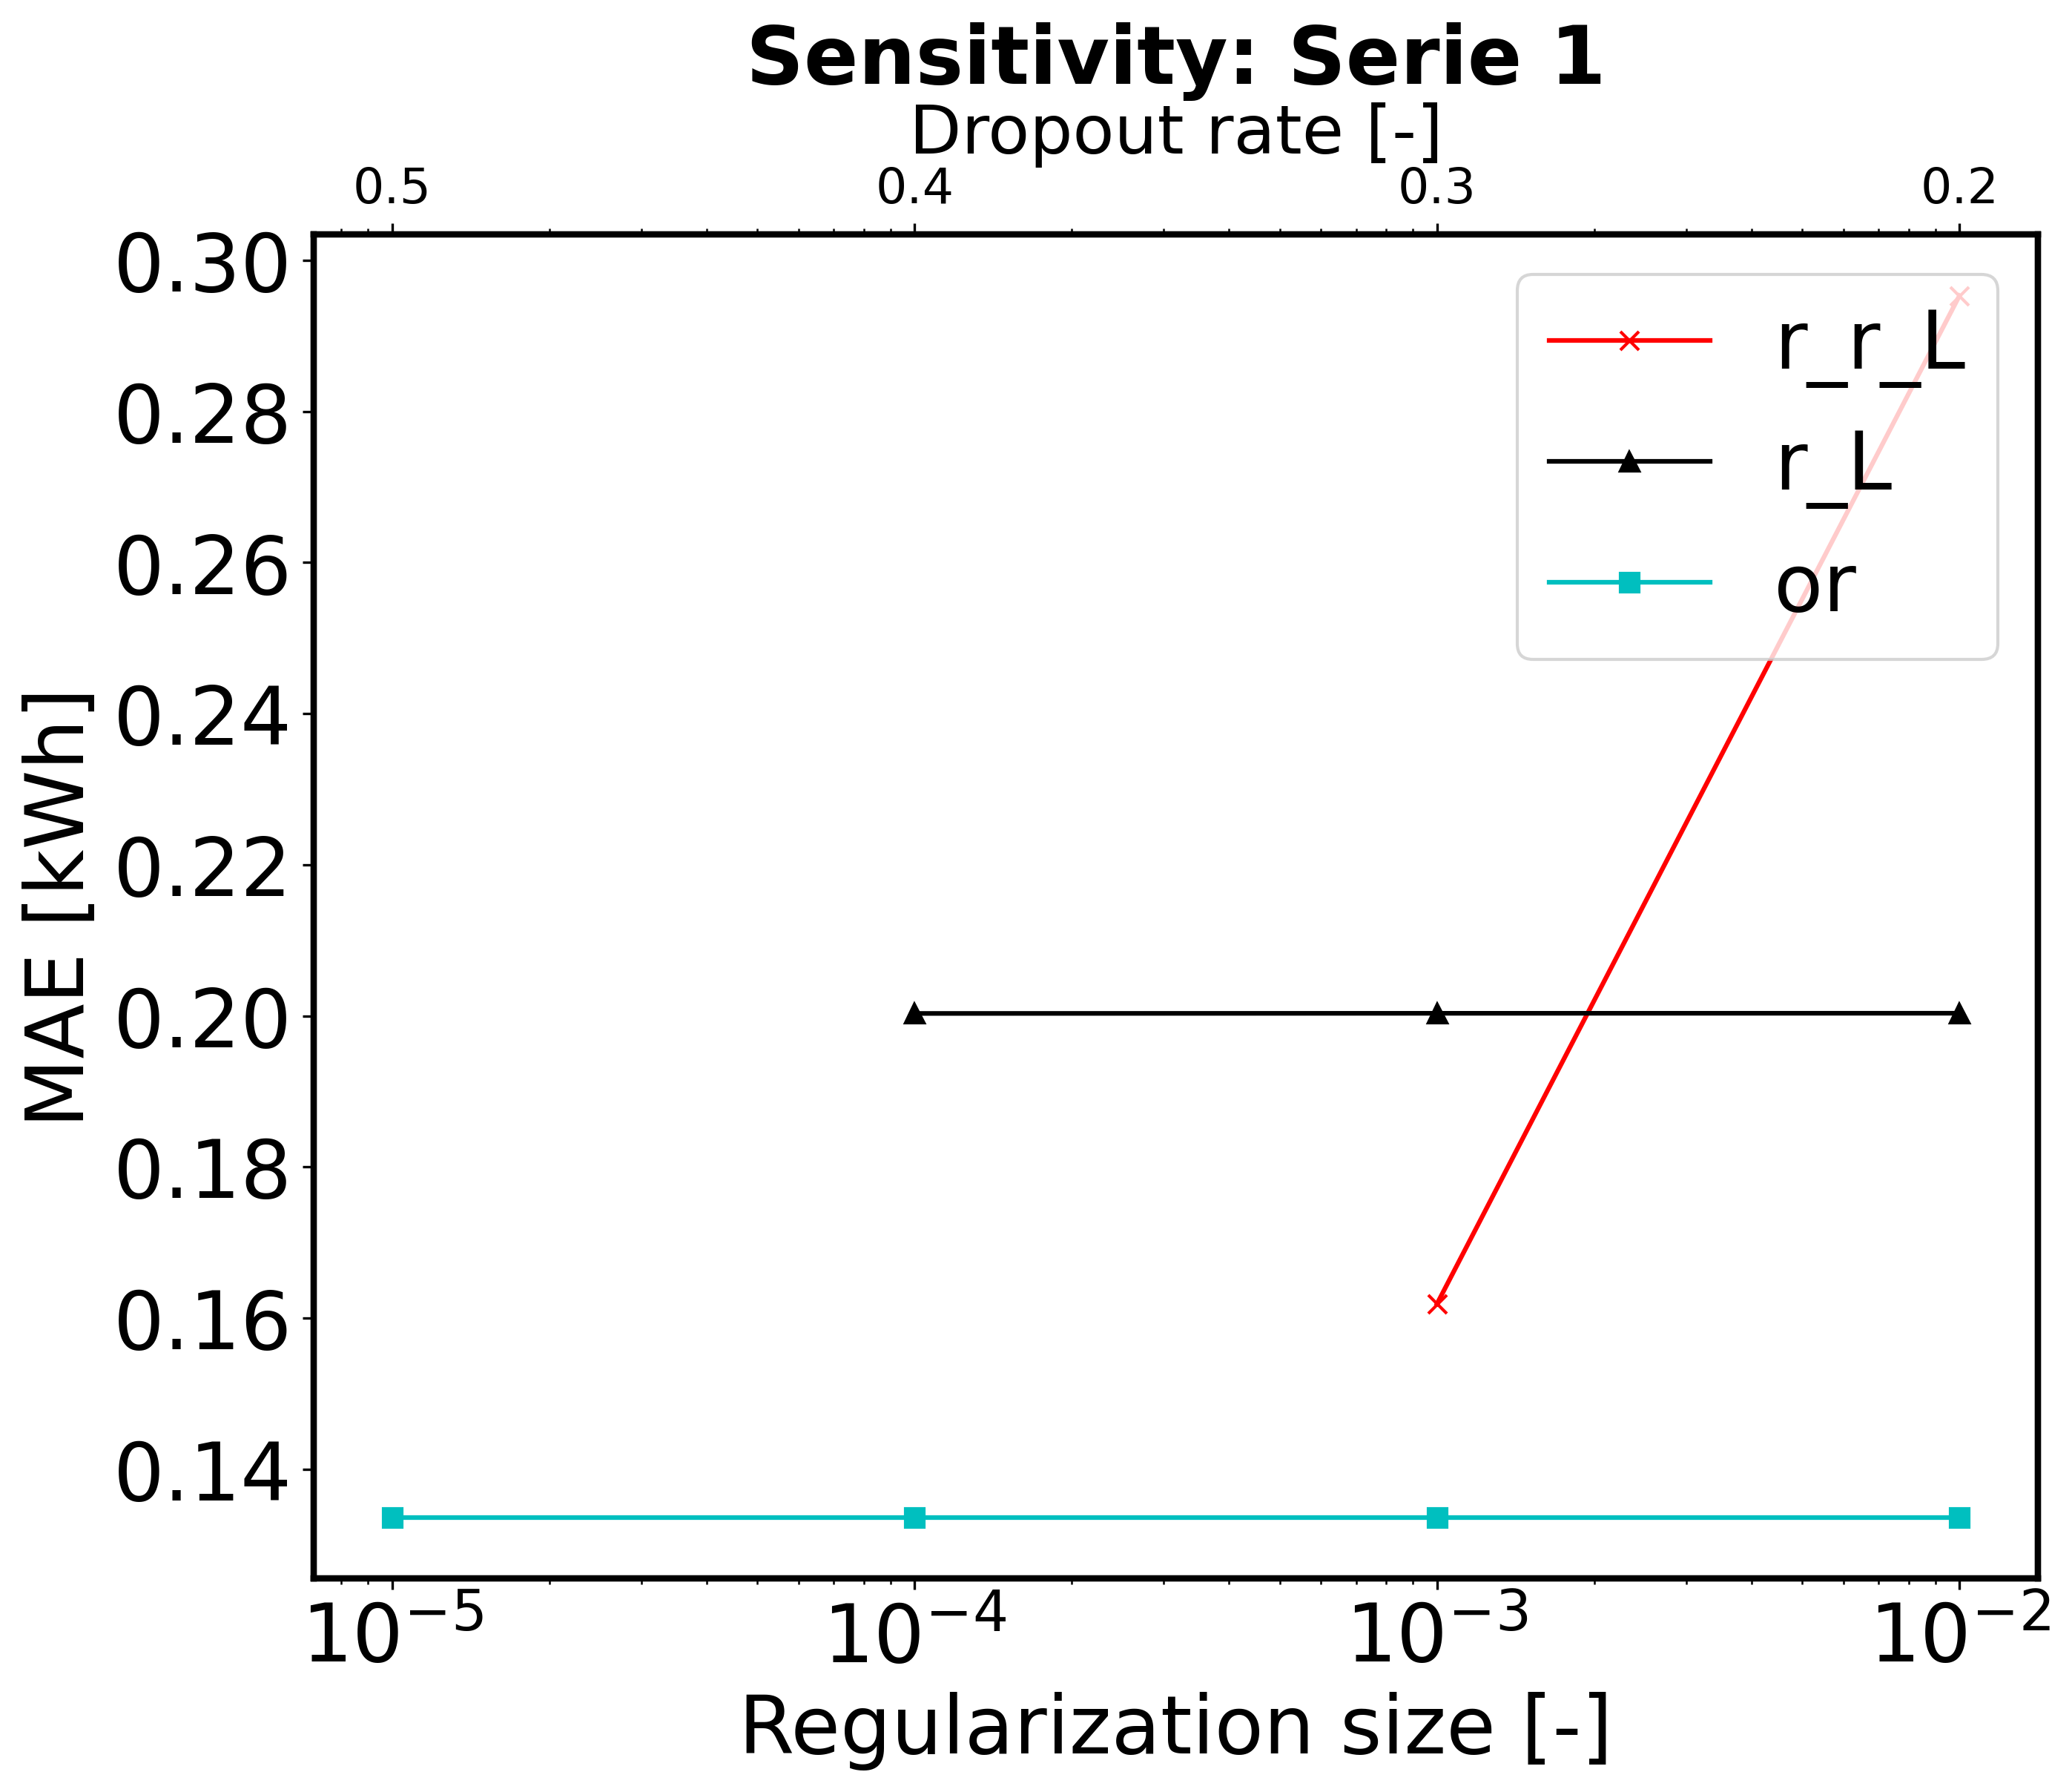
\includegraphics[width=1\linewidth]{serie1_model3.png}
		\caption{Model 3}
	\end{subfigure}	
	\begin{subfigure}{0.49\linewidth}
		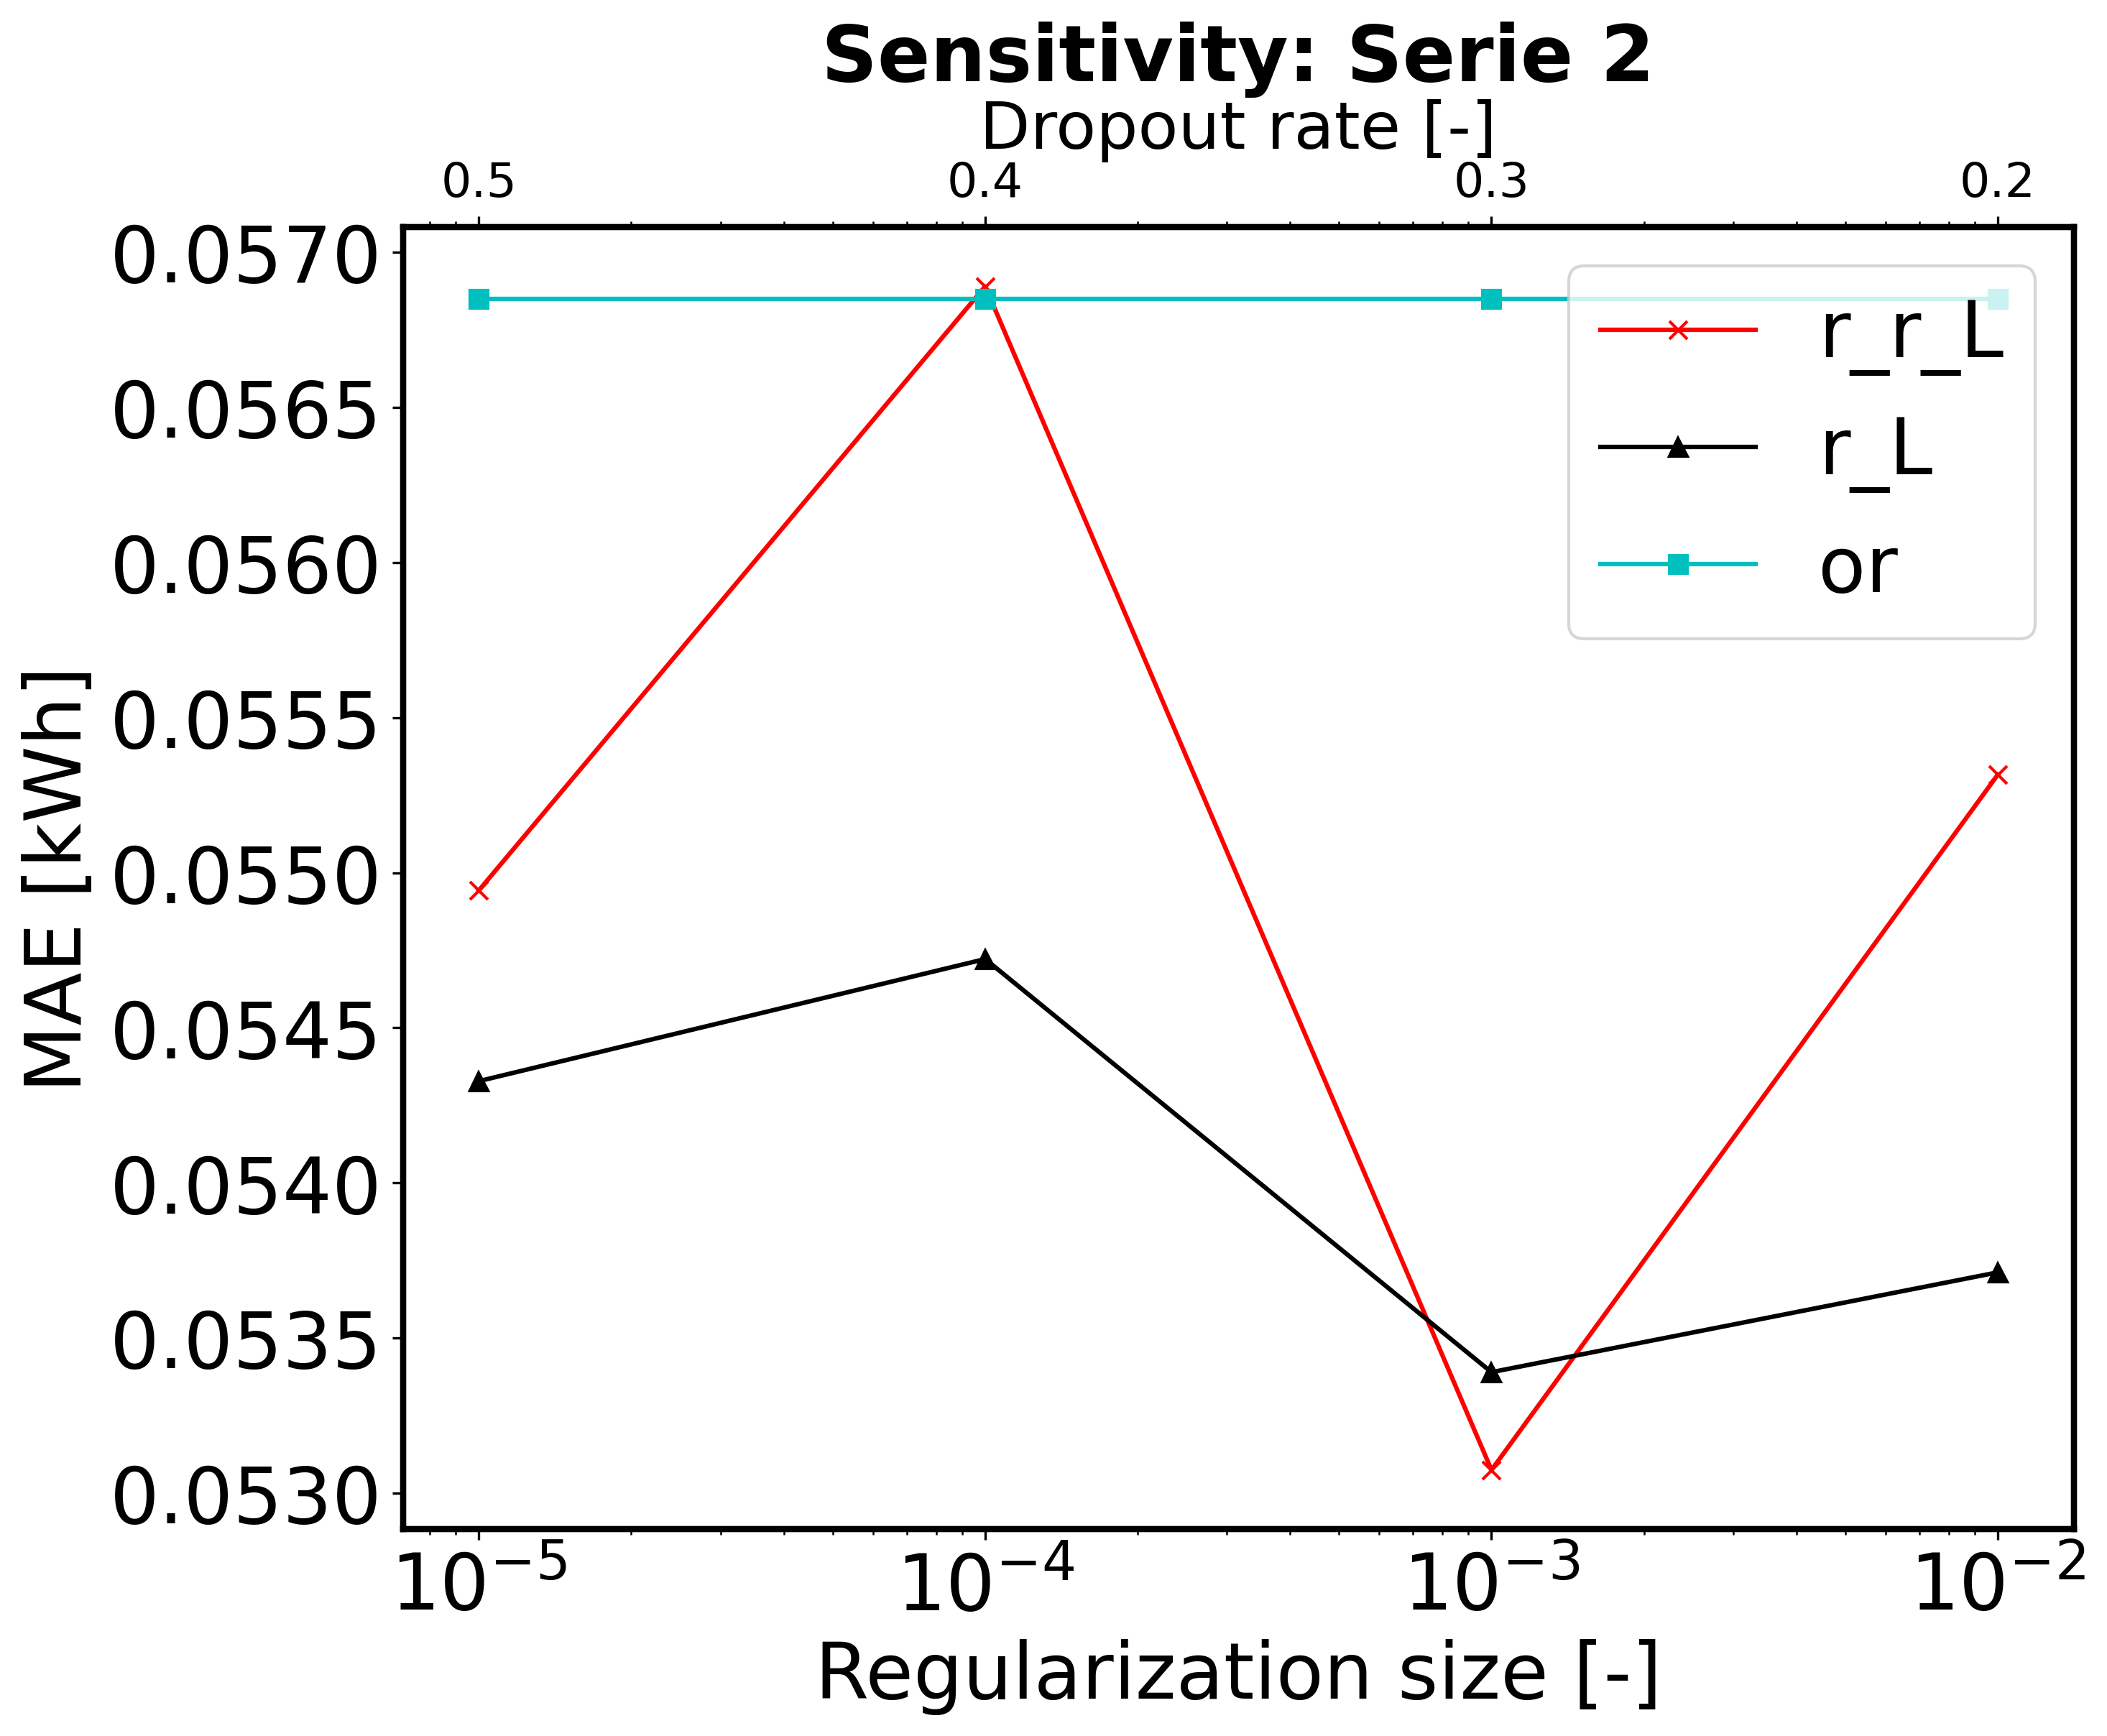
\includegraphics[width=1\linewidth]{serie2_model3.png}
		\caption{Model 3}
	\end{subfigure}
	\begin{subfigure}{0.5\linewidth}
		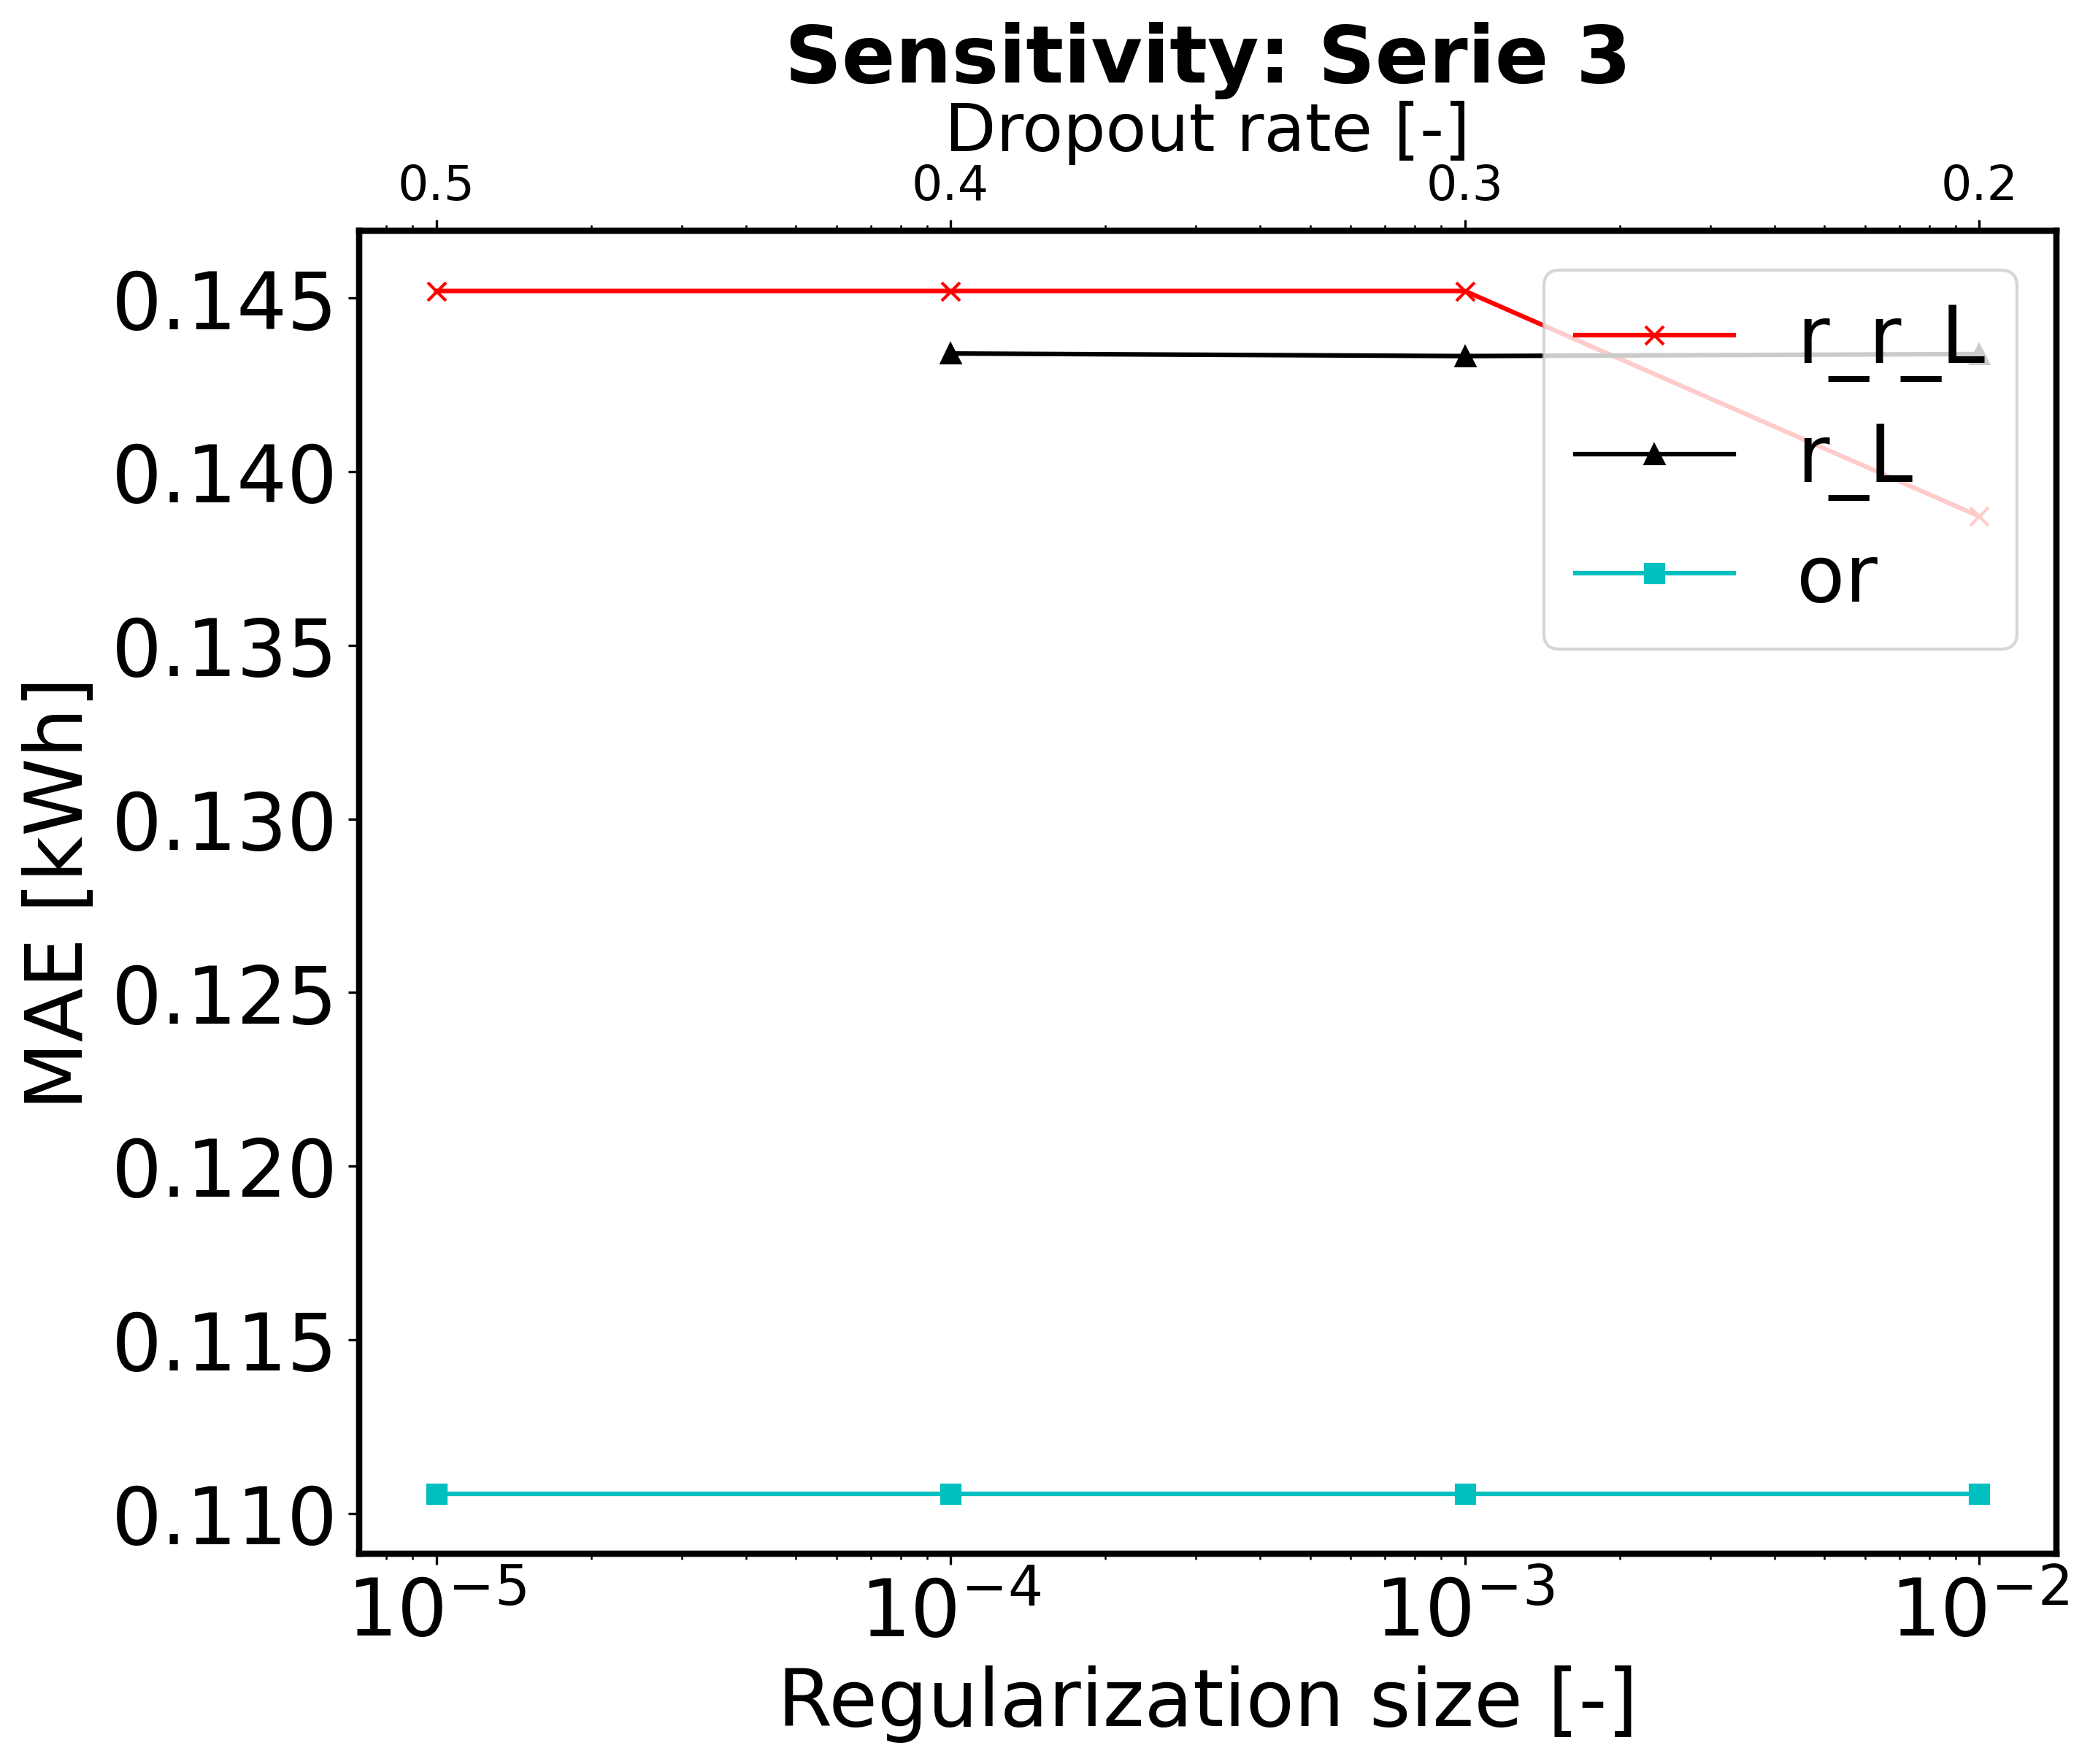
\includegraphics[width=1\linewidth]{serie3_model3.png}
		\caption{Model 3}
	\end{subfigure}
	\caption{Results of the sensitivity analysis on the size of regulation parameter and the dropout rate with respect to the mean absolute error.(Legend: \textit{r\_r\_L}: regularization size of recurrent weight of LSTM, \textit{r\_L}: regularization size of input weights of LSTM and \textit{or}: best performing serie from phase one)}
	\label{fig:sensitivity_model3}
\end{figure}

\begin{figure}[h]
	\centering
	\begin{subfigure}{0.49\linewidth}
		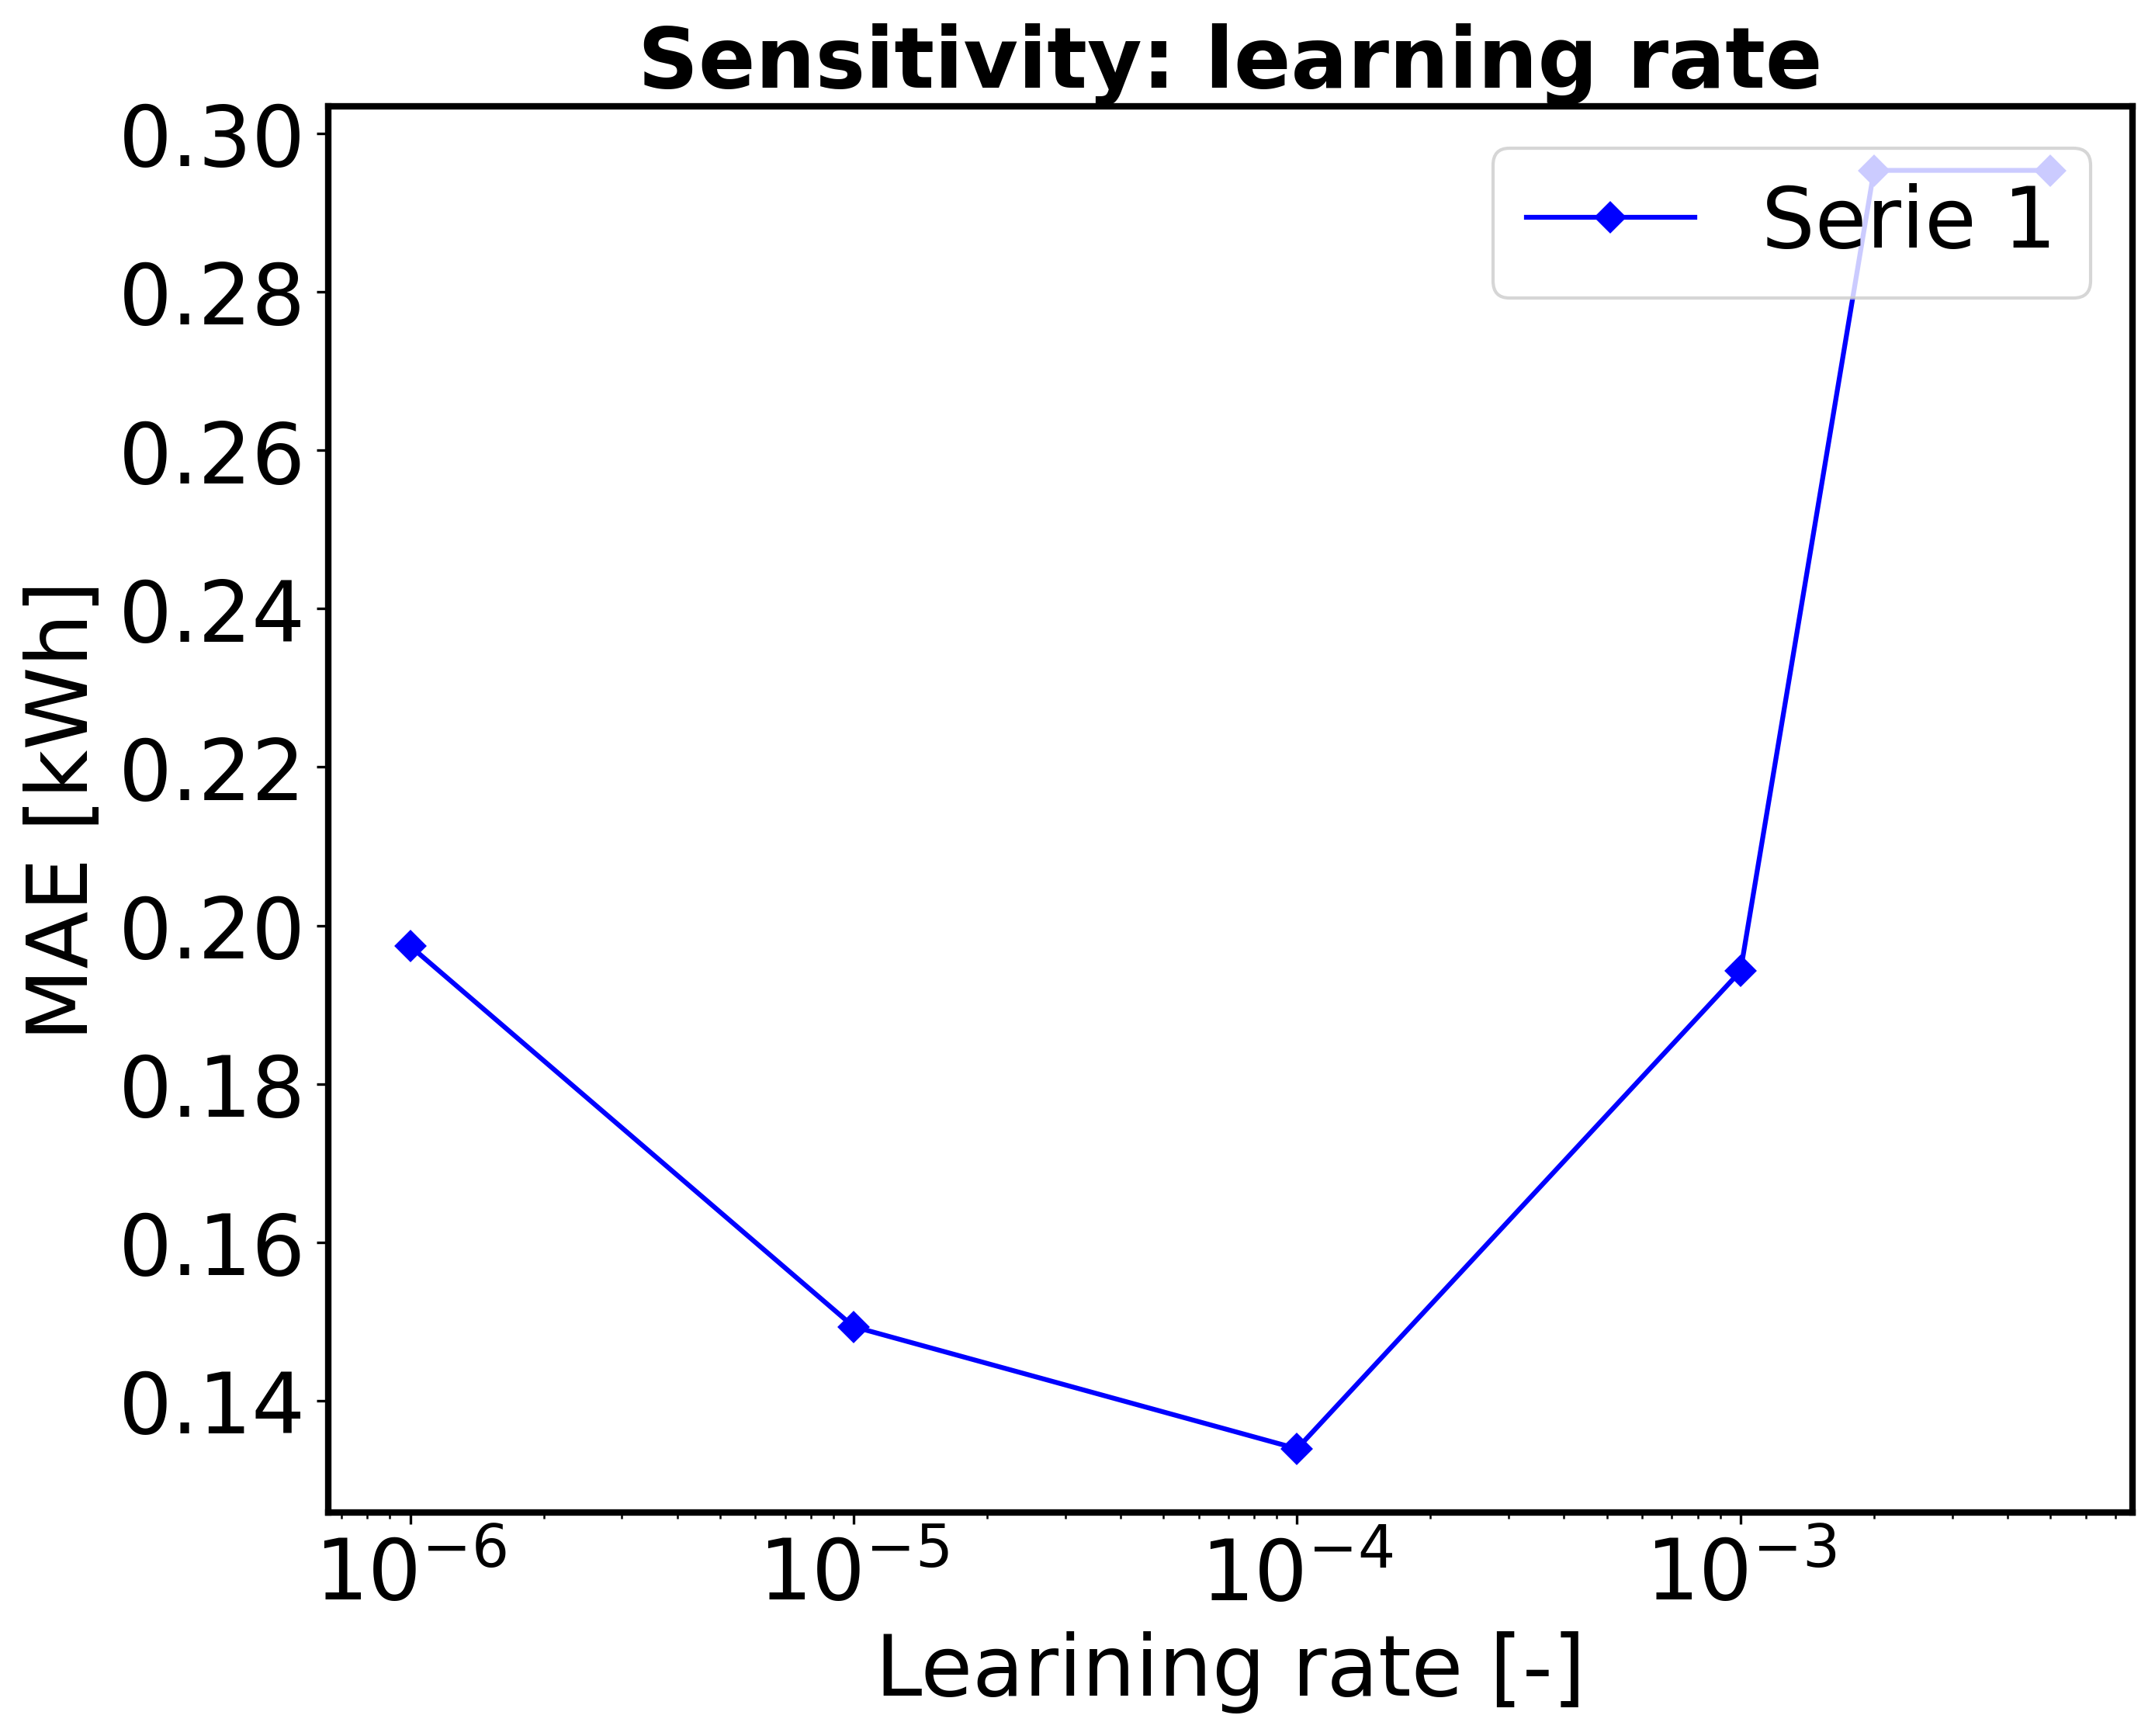
\includegraphics[width=1\linewidth]{learning_rate_serie1_model3.png}
		\caption{Model 3}
	\end{subfigure}	
	\begin{subfigure}{0.49\linewidth}
		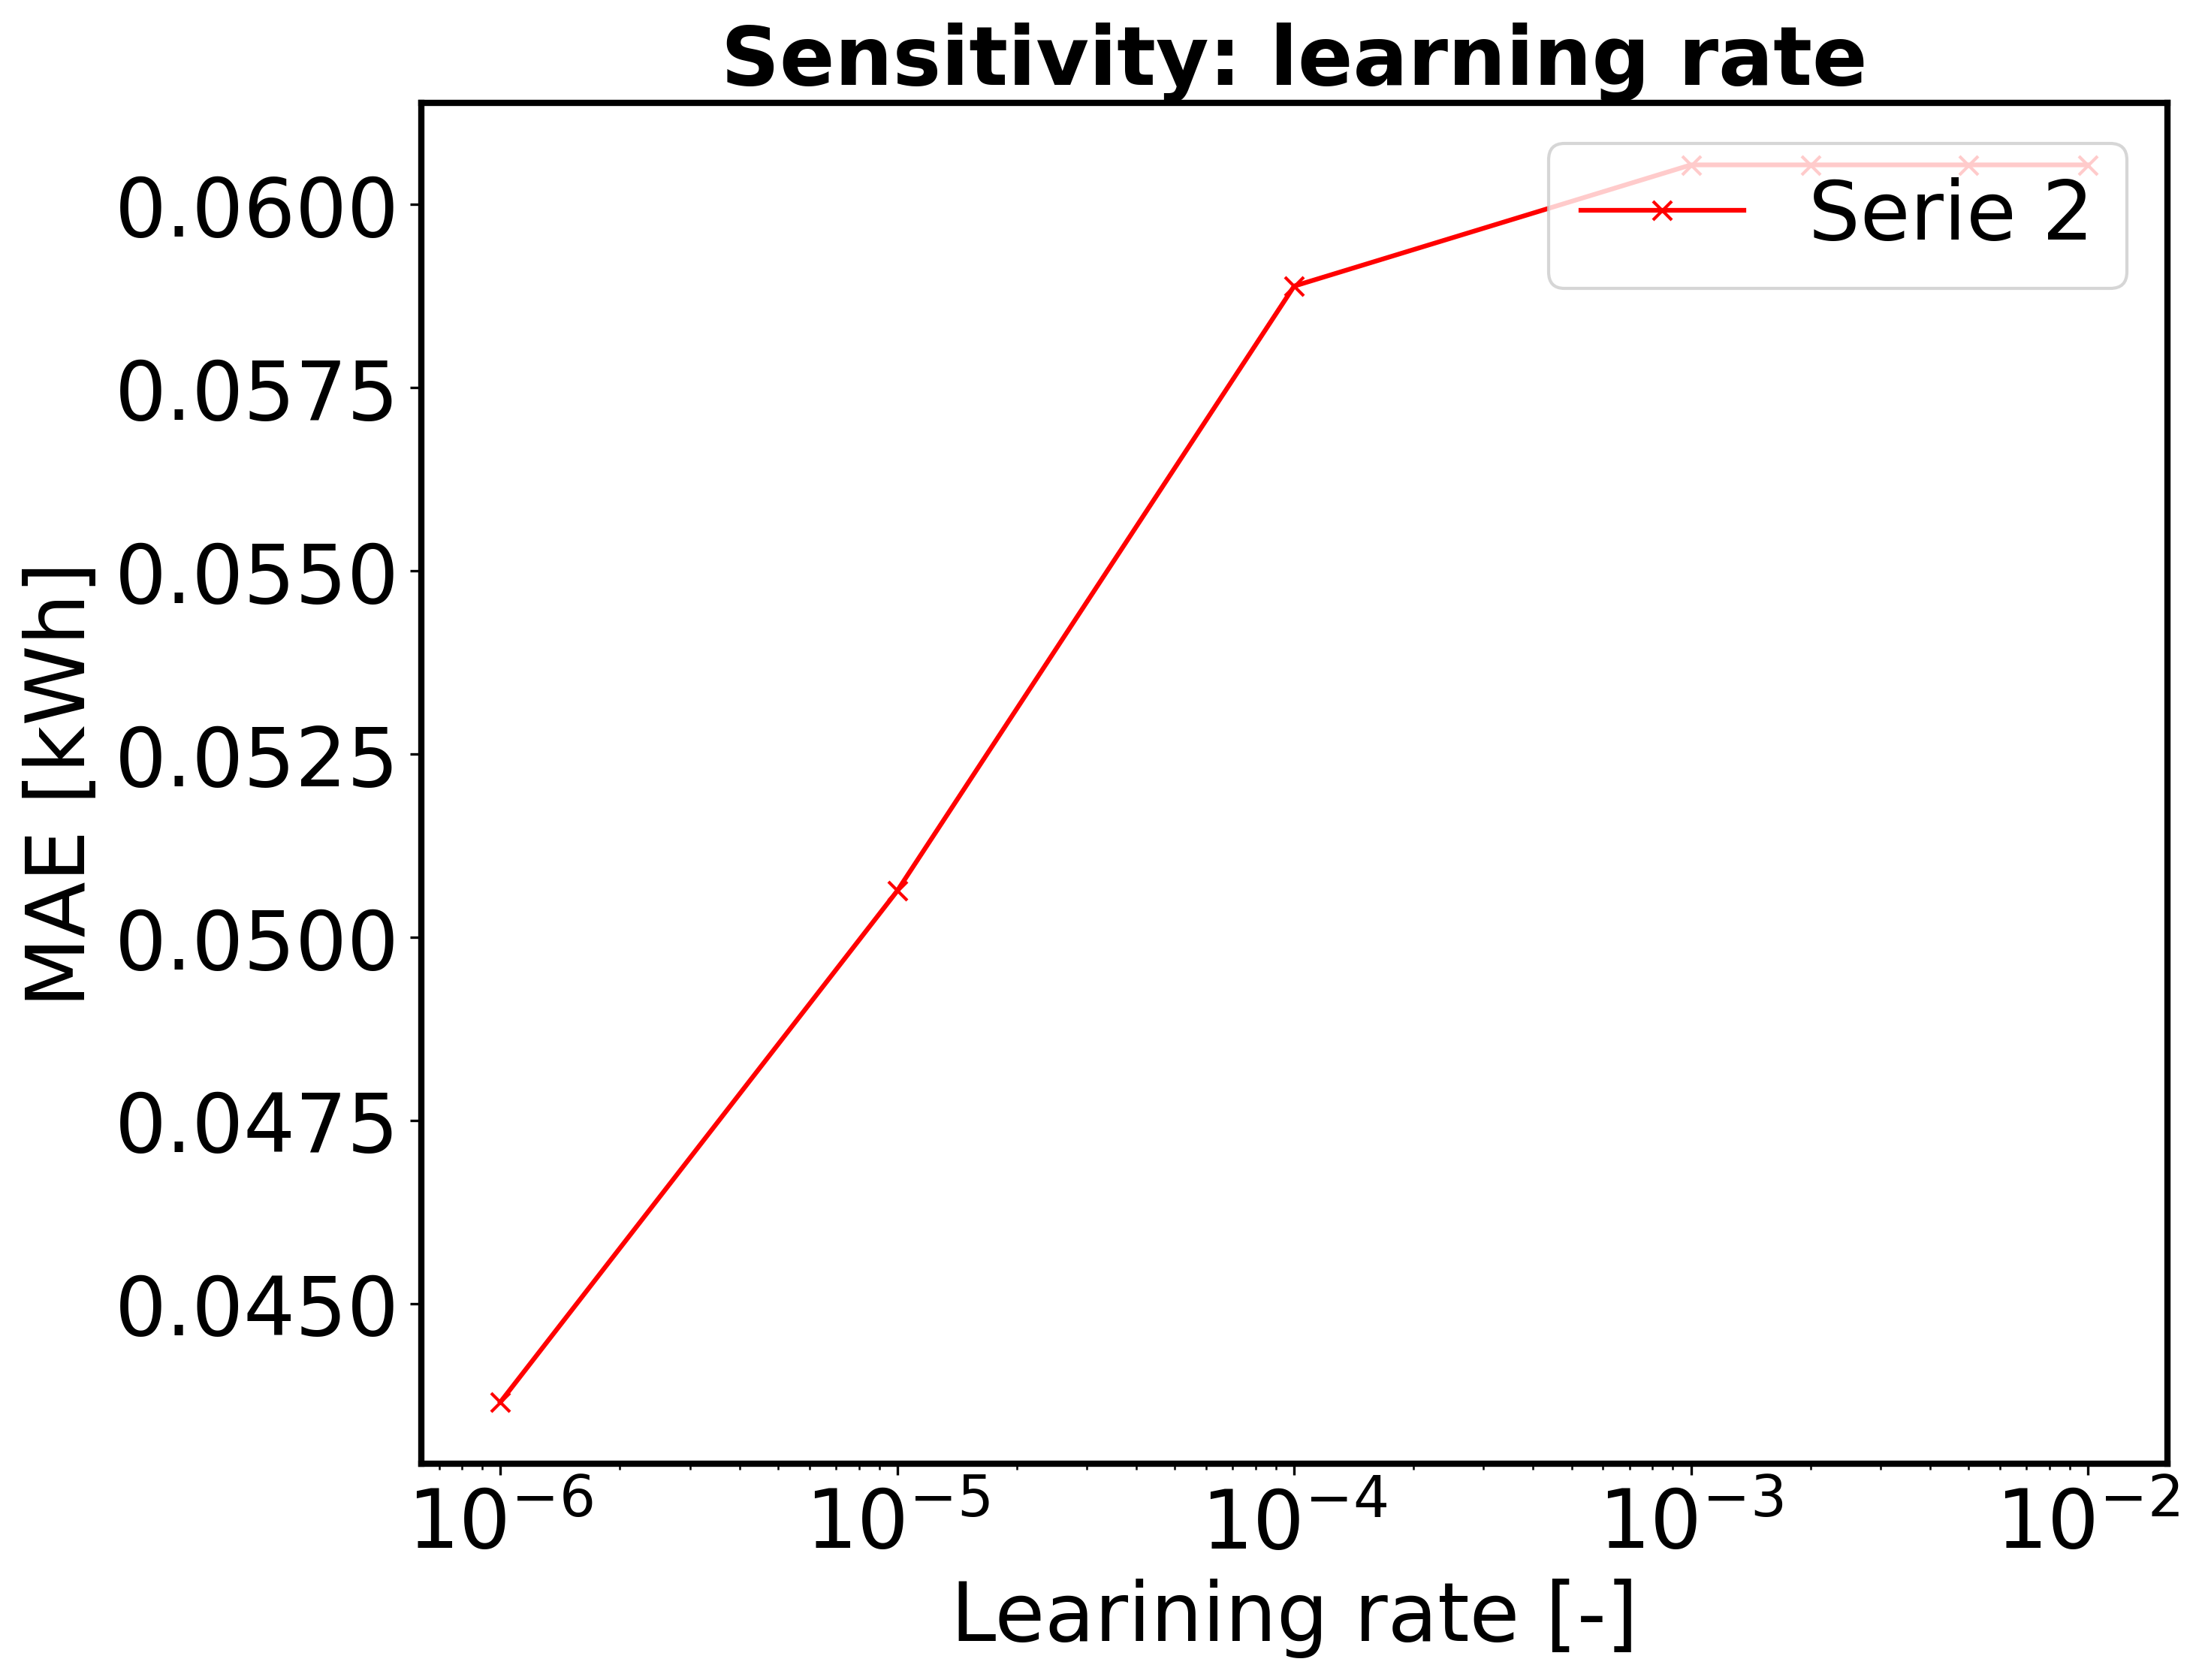
\includegraphics[width=1\linewidth]{learning_rate_serie2_model3.png}
		\caption{Model 3}
	\end{subfigure}
	\begin{subfigure}{0.5\linewidth}
		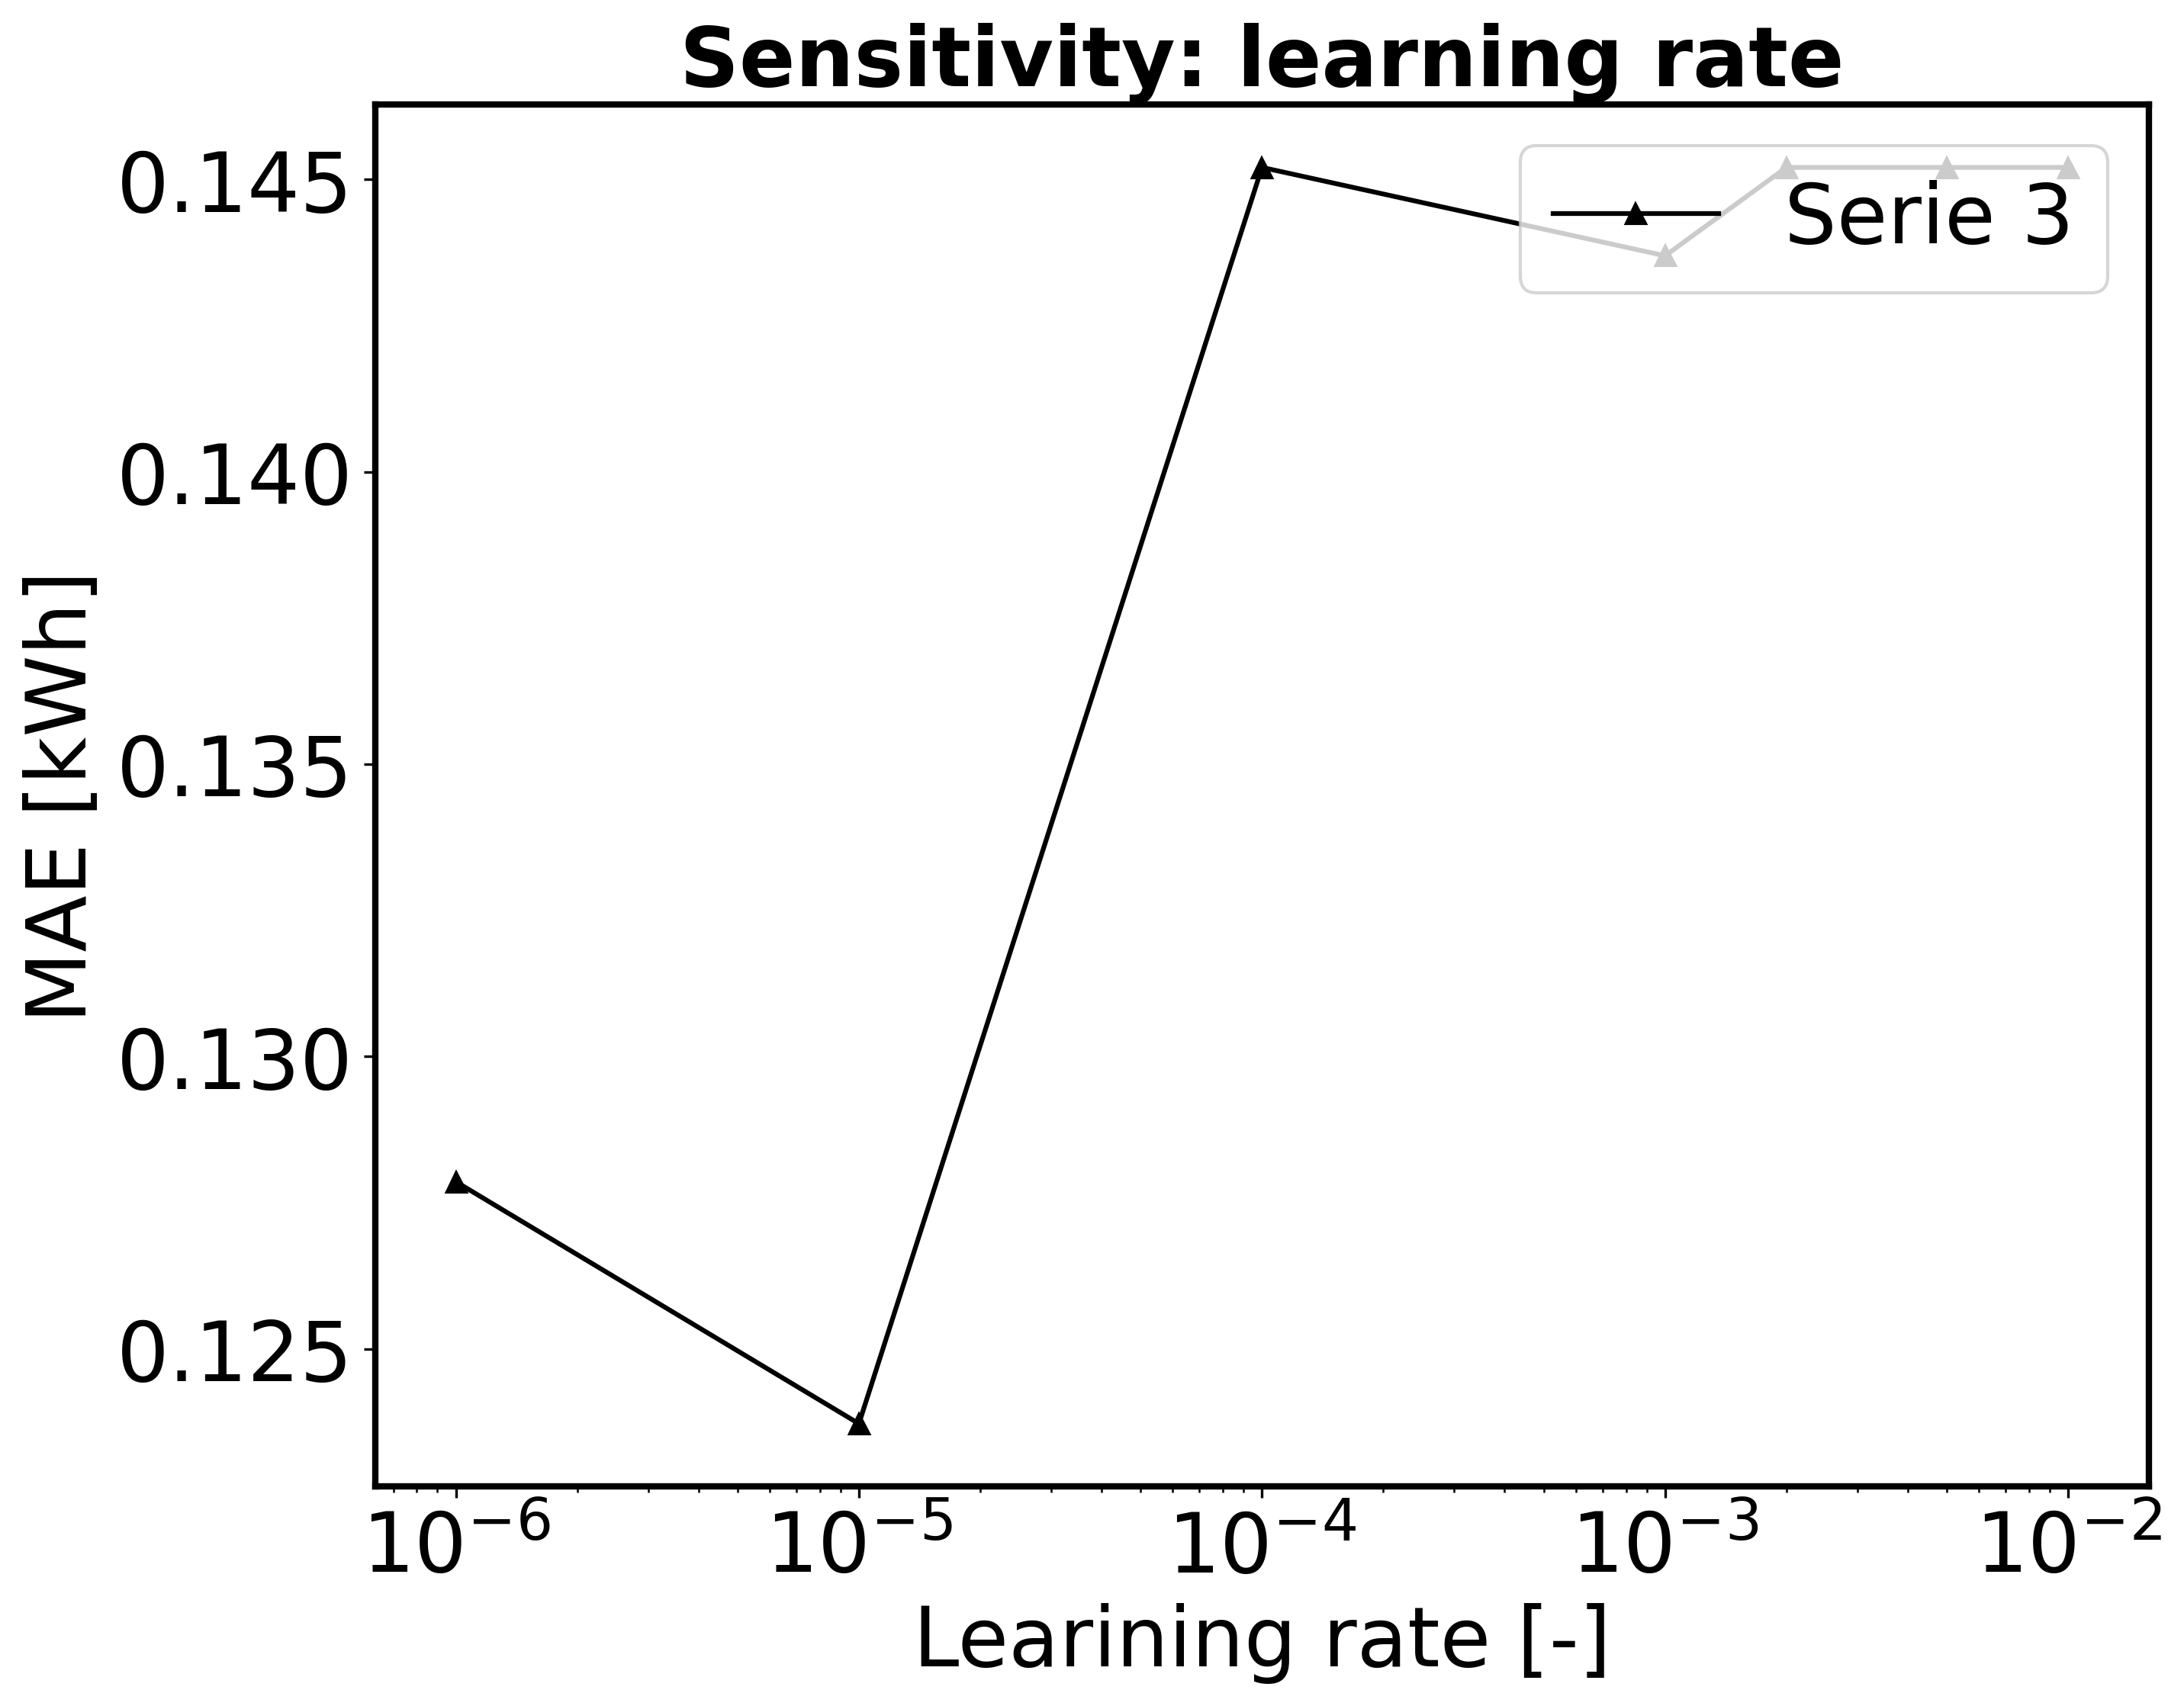
\includegraphics[width=1\linewidth]{learning_rate_serie3_model3.png}
		\caption{Model 3}
	\end{subfigure}
	\caption{The evaluation of the error on the validation set in function of the learning rate size.}
	\label{fig:learning_rate_model3}
\end{figure}





%%% Local Variables: 
%%% mode: latex
%%% TeX-master: "thesis"
%%% End: 
